\chapter{Gravitational Waves Theory and Detectors} % Write in your own chapter title
\label{Chapter One}
\section{Introduction}

Gravitational waves (GW) are waves in the space--time fabric and are a direct consequence of Albert Einstein's General Theory of Relativity. First introduced in 1916, gravitational waves had to wait for about six decades to have their physical existence confirmed in an indirect way (see the famous binary pulsar PSR1913+16, described below) and are still awaiting a direct detection.

Direct detection of gravitational waves is complicated by the extremely small effect they would produce on an Earth--based detector since the wave amplitude decreases inversely proportional with the distance to the source. Important progress has been made over the past twenty years with the commissioning of kilometer--scale interferometric \ac{GW} observatories, such as \ac{LIGO} (in the US) and the Virgo detector (in Italy). Constant upgrades to these detectors laid the path to advanced detectors to be commissioned within the next few years, that will achieve the first direct detection. Furthermore, space--based detectors such as \ac{LISA} will be the next big step up after the advanced \ac{LIGO} and Virgo. 

The capacity to detect \ac{GW} offers us the possibility to understand astrophysical systems that can not be observed in any wavelength of the electromagnetic spectrum. As an example, two black holes in a close binary system can not be observed in any way but by detecting the \ac{GW} they emit while inspiralling, observation that will provide us with information on their astrophysical parameters. With the first detection, the next few years will see the emergence of astronomy with \ac{GW}.

The main focus of this thesis is to describe a number data analysis techniques and challenges for detecting gravitational waves from \emph{compact binary coalescence} (CBC) events altogether with describing the available and planned tools for their detection, the \ac{GW} detectors. Before going into detail about the data analysis approaches, it is useful to give an overview of the theory behind \ac{GW}. In Chapter \ref{Chapter One} I will introduce the basic \ac{GW} theory, the sources of \ac{GW} radiation and the tools we have to make a detection, the \ac{GW} detectors.

Resembling electromagnetic radiation, gravitational waves carry away energy, angular momentum and linear momentum from the radiation source. They propagate at the speed of light $c$ and have two independent transverse polarization states (the $+$ and $\cross$ polarizations). Unlike electromagnetic waves, which are mainly dipolar radiation, gravitational waves are mainly quadrupolar radiation, the leading term in their generation being a time--varying mass quadrupole. There are no mass monopoles or dipoles involved in the radiation process and the contribution of octupoles and higher order multipole terms will be neglected in the calculations that follow.

The gravitational wave field is dimensionless, and its strength is qualitatively characterized by a single quantity called the gravitational wave amplitude or \emph{strain} $h$, a fractional change in length of any object that the wave passes through. The amplitude falls off during propagation from a localized source, in proportion to the inverse power of the traveled distance $h \propto D^{-1}$. The difficulty of direct detection of gravitational waves lies in that the expected amplitude (or strain in a GW detector) $h$, on Earth, from close--by astronomical sources is exceedingly small, of the order of, or smaller than $10^{-21}$ \cite{Schutz:2010xm}. The only way to prove the existence of gravitational waves is to measure this amplitude $h$ in the form of a strain applied by the wave on a series of test masses (see the {\it Detectors} section below).

\subsection{Gravitational waves sources}
We can distinguish a series of \ac{GW} sources according to the nature of their progenitor and the emitted waveform. These sources are likely to generate \ac{GW} with a large enough amplitude $h$ to be detected by present or upcoming \ac{GW} detectors.
 
\begin{itemize}
 \item{{\bf Transient sources}} Transient (or \emph{burst}) events are responsible for the release of a great amount of gravitational energy over a short period of time. It is believed that this type of signal will result from a short hard gamma-ray burst, the non--axial collapse of a supernova or even from a star crossing the event horizon of a black hole \cite{Blanchet:2004ek,Baker:2006yw,Ott:2006qp,Burrows:2005dv}. The search for such signals is unbiased by any theoretical assumptions and is performed without assuming any knowledge of the \ac{GW} waveform, therefore these types of sources are treated as {\it unmodelled}. The search will look for brief power excess events in the \ac{GW} detectors and given its unmodelled nature, may be able to discover new sources of \ac{GW} radiation \cite{Collaboration:2009kk,Abbott:2009zi,Abbott:2009zd,Abbott:2009up}  

 \item{{\bf Stochastic Background Radiation}} Similar to the cosmic microwave background (CMB) and the unprobed cosmic neutrino background, there exists a cosmic gravitational wave background. These gravitational waves are thought to have been emitted shortly after the Big Bang and they stretched as the universe expanded over time. Therefore they may be one of the best probes of the early universe. Other gravitational waves backgrounds could be created by the superposition of the radiation from all the cosmic sources, indistinguishable individually, but detectable as a whole. Observing such background radiation is promising since it would provide information on the physical properties of compact objects and their evolution with redshift, such as the mass of neutron stars or black holes, the ellipticity and the magnetic field of neutron stars, the angular momentum of black holes or the rate of compact binaries. For in--depth studies we refer the reader to \cite{Allen:1996vm,Abbott:2009ws,Abbott:2006zx,Abbott:2003hr, Regimbau:2011rp} and references therein.

 \item{{\bf Periodic Signals}} Periodic gravitational wave sources emit continuous, almost monochromatic waves, for very long intervals of time. Differential rotation of neutron stars (e.g., a symmetric spherical neutron star with a large mountain) can be tracked over many cycles to produce a periodic \ac{GW} signal \cite{Abbott:2008fx}. Through these observations, the gradual slowing of a pulsar spin (\emph{spin--down}) can be monitored. The waves can be used to monitor existing pulsars and search the sky to find new pulsars. The continuous wave sensitivity search is improved as the time of observation increases. An example of such a spin--down search using the Crab pulsar is presented in \cite{Abbott:2008fx}. This pulsar provides the best opportunity to detect continuous gravitational waves with
current gravitational wave interferometers. Assuming the \emph{in--extremis} case that the whole spin--down energy is converted into \ac{GW}, such a source would produce a gravitational strain amplitude of order $h \sim 1.4 \times 10^{-24}$. Although this value is too low for the detectors' capabilities, by observing the source for months or even years, the accumulation of power would be enough for a \ac{GW} detection. Since such a detection was not made, upper limits were placed that imply that less than 6$\%$ of the spin down energy of the Crab pulsar is emitted as gravitational waves. For a more in--depth analysis, we direct the reader to consult \cite{Jaranowski:1998qm,Collaboration:2009rfa,Abbott:2009nc,Abbott:2008rg} and references therein.   

 \item{{\bf \ac{GW} from Compact Coalescing Binaries}} Two compact stars orbiting each other around the common center of mass will lose energy and angular momentum due to emission of gravitational waves, gradually decreasing the separation between the components and increasing the orbital frequency. This process is known to be very lengthy (order of $\sim$Gyr) but the very last orbits before merger can be completed in very short times (fractions of seconds) and it is then when the bulk of gravitational waves energy is released. The signal detectable on Earth will be a {\it chirp wave} with a rapid increase in amplitude and frequency as the binary nears merger. This signal will be characterized by the binary masses and spins, radial separation and eccentricity of the two orbiting bodies. The search for gravitational waves from such objects is performed in a {\it modelled} way by analytically and numerically constructing the inspiral waveforms and matching the observational data with them. This \ac{GW} source is the main focus of this thesis and will be examined in detail in the following chapters.
\end{itemize}

\subsection{Observational evidence of \ac{GW}}

Unfortunately, there is no direct observation of gravitational waves as of yet, but there is a series of indirect proofs of their existence through astronomical observations of binary systems. The first such observation was brought by the discovery of the pulsar PSR B1913+16, observed by Russell Hulse and Joseph Taylor of Princeton University in 1974 \cite{Hulse:1974eb}. Both physicists have been awarded the Nobel Prize for Physics in 1993 for this discovery. PSR B1913+16 is a binary pulsar: one component is confirmed a millisecond pulsar with a period of 59 ms, whereas the other is inferred a neutron star by measuring the time of arrival of its companion's pulses. The separation between components has decreased over a span of 37 years in exact accordance with Einstein's theory of general relativity. According to this, the binary components lose energy and angular momentum due to emitting gravitational waves. Figure \ref{fig:hulsepulsar} is a diagram showing how exact is the relativistically predicted decrease (continuous line) compared to the actual data points. 

\begin{figure}[ht]
\centering
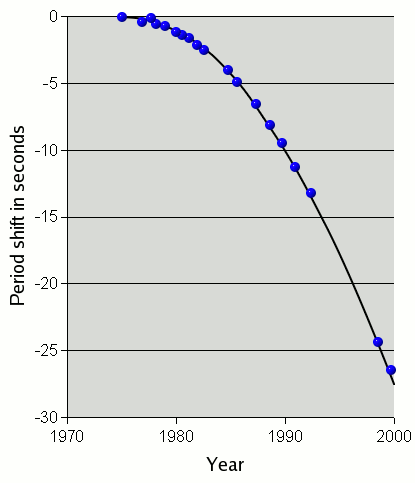
\includegraphics[scale=0.90]{Images/PSR.png}
\caption{The periastron period shift plotted against time, for the Hulse--Taylor PSR1913+16 binary pulsar. The companion arrives earlier at the periastron due to the decrease in separation, hence showing a decrease of the orbital period. Continuous line represents the predicted evolution due to emission of GW and the dots represent the observational data. The system is highly eccentric, and the losses in energy and angular momentum increase significantly as the eccentricity approaches one, i.e., as the ellipse of the orbit becomes more elongated. Image reproduced from \cite{Weisberg:2004hi}}
\label{fig:hulsepulsar}
\end{figure}

Another binary pulsar, PSR J0737--3039, shows the same decrease in orbital period due to \ac{GW} emission. Differently from PSR B1913+16, the components are both seen as pulsars and the orbital plane is almost face--on. This allows the dynamics of this system to be observed to a greater degree of accuracy than is possible with other binary systems and general relativity to be tested in a number of ways. Gravitational redshift and rate of change of the periastron could be accurately measured using data from PSR J0737--3039. All observations have been fully consistent with the predictions of general relativity \cite{Kramer:2006nb, Kim:2006fm}. In \cite{Kramer:2006nb} it is quoted that observations of this system agree with general relativity within an error of only 0.05\%.

An interesting example of indirect \ac{GW} observation is OJ 287, a BL Lacertae object that is believed to be a supermassive binary black hole system (SMBBH). The binary components are of asymmetric masses -- a supermassive black hole with a mass of $\sim 18 \times 10^9 M_{\odot}$ and a companion black hole with a mass of $\sim 10^8 M_{\odot}$. Since this object has been observed for almost 120 years, it was noticed that it displays a periodic variation in its visible magnitude that has a 12 year cycle with two outbursts at 12 year intervals. The supermassive black hole binary model would fit the observations as the system is modelled as the companion orbiting the primary on a moderately elliptical orbit, the emission peaks would occur as the companion's orbit intersects the primary's accretion disk. The times of the outbursts can be explained if the system emitted \ac{GW} \cite{Nature:0804, Sivaram:2008jy}.

\section{Linearized Gravity and Gravitational Waves}
 
Linearized gravity is an approximation in the study of general relativity in which the nonlinear contributions from the spacetime metric are ignored. This approach simplifies the calculations for many problems where approximate results can be used instead of the exact solutions. Linearized gravity is sometimes seen as flat space--time gravity with a small perturbation. One of the most important applications for linearized gravity is gravitational waves.

This section will give a brief overview of the theory behind \ac{GW}. We will focus on the linearized theory of \ac{GW} as described in \cite{MTW, Sch85, Maggiore:gw, 1999physics8041C}. We will closely follow the formalism and workflow given in these references. Therefore, this section will serve as foundation for the other chapters but is not intended as an in--depth description of the \ac{GW} theory, and we point the reader to consult the above mentioned references for a comprehensive analysis.

\subsection{Einstein's field equations and the weak--field approximation}
Einstein's field equations are a set of ten equations that describe quantitatively Einstein's theory of general relativity. They define gravity in terms of the curvature of space--time due to presence of matter and energy. In the standard tensor notation they are given by:
%
\begin{equation}
\label{eq:einsteins}
G_{\mu \nu} = R_{\mu \nu} - \frac{1}{2} g_{\mu\nu}R = \frac{8\pi G}{c^4} T_{\mu \nu} 
\end{equation}
%
where $R_{\mu \nu}$ is the Ricci tensor, $R$ the Ricci scalar and $g_{\mu\nu}$ the metric tensor of four--dimensional space--time. The Riemannian curvature tensor is defined as
\begin{equation}
R^{\mu}_{~\gamma\alpha\nu} = \frac{\partial \Gamma^{\mu}_{~\alpha\gamma}}{\partial x^{\nu}} - \frac{\partial \Gamma^{\mu}_{~\nu\gamma}}{\partial x^{\alpha}} + \Gamma^{\mu}_{~\nu\beta}~\Gamma^{\beta}_{~\alpha\gamma} - \Gamma^{\mu}_{~\alpha\beta}~\Gamma^{\beta}_{~\nu\gamma}
\end{equation} 
%
where $\Gamma$ is the {\it Christoffel symbol} or the {\it affine connection} defined as: 
\begin{equation}
\Gamma^{\mu}_{~~\alpha\beta} = \frac{1}{2} g^{\mu\nu}\left(
\frac{\partial g_{\nu\alpha}}{\partial x^{\beta}} +
\frac{\partial g_{\beta\nu}}{\partial x^{\alpha}} -
\frac{\partial g_{\alpha\beta}}{\partial x^{\nu}}\right)
\end{equation}
%
The Ricci tensor is:
%
\be R_{\mu \nu} = R^{\alpha}_{\mu\alpha\nu} \ee
%
and the Ricci scalar is:
%
\be R = g^{\mu \nu}R_{\mu\nu}, \ee
%
In a ``flat'' space,
%
\begin{equation}
R^{\mu}_{~\gamma\alpha\nu} = 0.
\end{equation}
%
$T_{\mu \nu}$ is the stress energy tensor, which describes the density and flux of matter (or energy) and momentum. The components of this tensor may be interpreted in the following way, according to \cite{Sch85}:
%
\begin{itemize}
 \item $T_{00}$ is the energy (or relativistic mass) density.
 \item $T_{0i} = T_{i0}$ is the energy flux in the $i$--th direction, or the density of $i$--momentum.
 \item $T_{ij}$ is flux of $i$--momentum in the $j$--th direction.
\end{itemize}
%
Einstein's equations describe ten equalities, rather than the 16 apparent. This is
because $R_{\mu\nu}$, $g_{\mu\nu}$ and $T_{\mu\nu}$ are all symmetric.

Gravitational waves may be naively seen as {\it ripples} in the space--time fabric created by a strong gravitational field source. Our analysis follows the weak--field approximation, therefore we place the observer far away from the putative source. We will consider that the gravitational field at the observer is \emph{weak} but not \emph{static}. Also, consider that there are no restrictions on the motion of particles in the vicinity of the observer. In the absence of gravitational interaction, space--time is flat and is characterized by the Minkowski flat metric \cite{1999physics8041C}:
%
\begin{equation}
\eta = \left( \begin{array}{cccc}
           -1 & 0 & 0 & 0 \\
	    0 & 1 & 0 & 0 \\
	    0 & 0 & 1 & 0 \\
            0 & 0 & 0 & 1 \end{array} \right)
\end{equation}
%
A weak gravitational field can be considered as a small ``perturbation'' on the flat Minkowski metric \cite{MTW,Sch85,Maggiore:gw},
%
\begin{equation}
g_{\mu\nu} = \eta_{\mu\nu} + h_{\mu\nu}, ~~~||h_{\mu\nu}|| \ll 1
\end{equation}

\noindent The condition $||h_{\mu\nu}|| \ll 1$ shows that the analysis is done in a weak gravitational field. Here $||h_{\mu\nu}||$ is defined as the magnitude of a typical non--zero component of $h_{\mu\nu}$. In linearized gravity, the smallness of the perturbation means that we only keep terms which are linear in $h_{\mu\nu}$ (approximation to first order), higher order terms are discarded. As a consequence, indices are raised and lowered using the flat metric $\eta_{\mu\nu}$ . The metric perturbation $h_{\mu\nu}$ transforms as a tensor under Lorentz transformations. We can therefore write,

\begin{equation}
g^{\mu\nu} = \eta^{\mu\nu} - h^{\mu\nu}
\end{equation}

Under a background Lorentz transformation \cite{Sch85}, the perturbation 
transforms as a second--rank tensor:

\begin{equation}
h_{\alpha\beta} = \Lambda_{\alpha}^{~~\mu} \Lambda_{\beta}^{~~\nu} ~h_{\mu\nu}
\end{equation}

The equations obeyed by the perturbation, $h_{\mu\nu}$, are obtained by
writing Einstein's equations to first order. To first order, the 
Christoffel symbol is \cite{MTW,Sch85,Maggiore:gw},

\begin{equation}
\Gamma^{\lambda}_{~~\mu\nu} = \frac{1}{2} \eta^{\lambda\rho}[\partial_{\mu}
h_{\rho\nu} + \partial_{\nu}h_{\mu\rho} - \partial_{\rho}h_{\mu\nu}] + 
{\cal{O}}(h^2)
\end{equation} 

Therefore, the Riemann curvature tensor will reduce to

\begin{equation}
R_{\mu\nu\rho\sigma} = \eta_{\mu\lambda}\partial_{\rho}\Gamma^{\lambda}_{~\nu\sigma} - \eta_{\mu\lambda}\partial_{\sigma}\Gamma^{\lambda}_{~\nu\rho}
\end{equation}

The Ricci tensor is obtained to first order in $h$:

\begin{equation}
R_{\mu\nu} \approx R^{(1)}_{\mu\nu} = \frac{1}{2}\left[\partial_{\lambda}\partial_{\nu}h^{\lambda}_{~\mu} + \partial_{\lambda}\partial_{\mu}h^{\lambda}_{~nu} - \partial_{\mu}\partial_{\nu}h - \Box h_{\mu\nu}\right]
\end{equation}
%
where, $\Box = \eta^{\lambda\rho}\partial_{\lambda}\partial_{\rho}$ is 
the D'Alembertian in flat space--time. Contracting with $\eta^{\mu\nu}$,
the Ricci scalar is:

\begin{equation}
R = \partial_{\lambda}\partial_{\mu} h^{\lambda\mu} - \Box h
\end{equation}
%
The Einstein tensor, $G_{\mu\nu}$, in the limit of weak gravitation is given by:

\begin{equation}
G_{\mu\nu} = R_{\mu\nu} - \frac{1}{2} \eta_{\mu\nu} R = \frac{1}{2}[\partial_{\lambda}\partial_{\nu}h^{\lambda}_{\mu} + \partial_{\lambda}\partial_{\mu}h^{\lambda}_{~\nu} - \eta_{\mu\nu}\partial_{\mu}\partial_{\nu}h^{\mu\nu} + \eta_{\mu\nu}\Box h - \Box h_{\mu\nu}]
\label{infnsol}
\end{equation}
%
For simplicity one can choose geometric coordinates $c=G=1$. 

Equation set (\ref{infnsol}) will have an infinite number of solutions. The decomposition of $g_{\mu\nu}$ in the weak gravitational field approximation does not completely specify the coordinate system in space--time. In solving Einstein’s equations it is common practice to impose gauge conditions: one adds new conditions on the metric tensor until the coordinate system is uniquely fixed. After four gauge conditions are imposed (the number of degrees of freedom in choosing the coordinate system), the metric is determined.
When we have a system that is invariant
under a gauge transformation, we {\it fix} the gauge and work in a selected 
coordinate system. One such coordinate system is the Lorentz gauge coordinate system, the gauge in which linearized gravity is simplest \cite{1999physics8041C, Maggiore:gw}. The gauge condition is called {\it Lorentz gauge}:
%
\begin{equation}
g^{\mu\nu}\Gamma^{\lambda}_{~~\mu\nu} = 0 
\end{equation}
%
In the weak field limit, this condition reduces to 
%
\begin{equation}
\partial_{\lambda} h^{\lambda}_{~~\mu} = \frac{1}{2}\partial_{\mu} h
\end{equation}
%
In this chosen gauge, the linearized Einstein equations simplify to:
%
\begin{equation}
\Box h_{\mu\nu} - \frac{1}{2} \eta_{\mu\nu}\Box h = - 16 \pi G T_{\mu\nu}
\end{equation}
%
The trace--reversed perturbation, $\bar{h}_{\mu\nu}$, is defined as follows:
%
\begin{equation}
\bar{h}_{\mu\nu} = h_{\mu\nu} - \frac{1}{2}\eta_{\mu\nu} h
\end{equation}
%
The Lorentz gauge condition further reduces to:
%
\begin{equation}
\partial_{\mu} \bar{h}^{\mu}_{~\lambda} = 0
\end{equation}
%
The Einstein equations are then:
%
\begin{equation}
\Box \bar{h}_{\mu\nu} = - 16 \pi G T_{\mu\nu}
\end{equation}
%
The above equation is written in the presence of matter and energy. If written in vacuum, 
where the stress--energy tensor will vanish, we obtain the familiar plane waves equation:
%
\begin{equation}
\Box \bar{h}_{\mu\nu} = 0
\end{equation}
%
The vacuum equations for $\bar{h}_{\mu\nu}$ are similar to the wave 
equations in electrodynamics or acoustics. 
These second order partial differential equations will have plane--wave solutions of the type:
%
\begin{equation}
\bar{h}_{\mu\nu} = B_{\mu\nu} {\rm e}^{i k_{\alpha}x^{\alpha}}
\label{hsolution}
\end{equation}
%
where, $B_{\mu\nu}$ is a constant, symmetric second rank tensor and $k_{\alpha}$
is a constant four--vector known as the {\it plane wave vector} satisfying 
%
\begin{equation}
k_{\alpha}k^{\alpha} = 0
\end{equation}
%
This shows that a solution (\ref{hsolution}) is possible
if $k_{\alpha}$ is {\it null} -- tangent to the world line of a
photon, i.e., gravitational waves propagate at the speed of light $c$ in vacuum. Since we used the $c=G=1$ notation convention, it is not straightforward to see that, in fact,  $c$ is a conversion factor used in order to change the units of time to units of space. This makes it the only speed which does not depend either on the motion of an observer or of a gravitational waves source, therefore $c$ is also the speed of gravitational waves and any other massless particle (like the photon). The time--like component of the wave vector is referred to as the 
{\it frequency} of the wave. The four--vector, 
$k_{\alpha}$ is usually written as $k_{\alpha} \equiv (\omega, {\bf k})$.
%
\begin{equation}
\omega_{gw}^2 = |{\bf k}|^2
\end{equation}
%
This represents the {\it dispersion relation} for the 
gravitational waves. The plane wave is completely described by a number of 
independent parameters: ten from the coefficients $B_{\mu\nu}$ and three 
from the null vector $k_{\alpha}k^{\alpha} = 0$.

\subsection{Transverse traceless gauge}
We use the Lorentz gauge to prove that that gravitational radiation
will propagate in vacuum as transverse plane waves at the speed of light $c$. There
are, however, further gauge freedoms that can be used to further simplify the form
of $h_{\mu\nu}$ . Using the Lorentz gauge condition, one obtains as follows:
%
\begin{equation}
k_{\alpha} B^{\alpha\beta} = 0 
\end{equation}
%
This imposes a restriction on $B^{\alpha\beta}$ : it is orthogonal 
({\it transverse}) to $k_{\alpha}$. The number of independent 
components of $B_{\alpha\beta}$ is thus reduced to six.
It can be easily proved that any coordinate transformation of the form
%
\begin{equation}
x^{\alpha^{\prime}} = x^{\alpha} + \xi^{\alpha}(x^{\beta})
\end{equation}
%
will leave the plane wave equation
%
\begin{equation}
\Box x^{\mu} = 0
\end{equation}
%
satisfied as long as
%
\begin{equation}
\Box \xi^{\alpha} = 0
\end{equation}
%
One can therefore choose a solution
%
\begin{equation}
\xi_{\alpha} = C_{\alpha} {\rm e}^{i k_{\beta} x^{\beta}}
\end{equation}
%
to the wave equation for any $\xi_{\alpha}$. $C_{\alpha}$ are constant 
coefficients. If
%
\begin{equation}
B^{\mu}_{\mu} = 0 ~~~~({\rm \it traceless})
\end{equation}
%
and
%
\begin{equation}
B_{\mu\nu} V^{\beta} = 0
\end{equation}
%
where, $V^{\beta}$ is some fixed four--velocity, that is, any constant 
time dependent unit vector one wishes to choose. The equations
%
\begin{equation}
k_{\alpha} B^{\alpha\beta} = 0 \hspace{1cm}
B^{\mu}_{\mu} = 0 \hspace{1cm}
B_{\mu\nu} V^{\beta} = 0
\end{equation}
%
are called the the {\it transverse--traceless} (TT) gauge 
conditions \cite{Sch85}. The trace condition $B^{\mu}_{\mu} = 0$ implies that
%
\begin{equation}
\bar{h}^{TT}_{\alpha\beta} = h^{TT}_{\alpha\beta}
\end{equation}


Consider now a background Lorentz transformation in
which the vector $V^{\alpha}$ is the time basis vector $V^{\alpha} = 
\delta^{\alpha}_{~0}$. Then the third TT equation implies that $B_{\mu 0} = 0$ for all
$\mu$. Further consider a privileged orientation of the coordinate axes so that the wave is travelling 
along the $z$-direction, $k^{\mu} \rightarrow (\omega_{gw}, 0, 0, \omega_{gw})$. 
Then with the TT equations it implies that $B_{\alpha z} = 0$ for all
$\alpha$. The $xx$ and $xy$ components of the amplitude tensor are also called the polarizations and labelled as $xx \equiv +$ and $xy \equiv \times$ as in the following ~\cite{Maggiore:gw, 1999physics8041C}:

\begin{equation}
B^{TT}_{\alpha\beta} = \left( \begin{array}{cccc}
              0 & 0 & 0 & 0 \\
              0 & B_+ & B_{\times} & 0 \\
              0 & B_{\times} & -B_{+} & 0 \\
              0 & 0 & 0 & 0 \end{array} \right)
\label{eqn:polarizations}
\end{equation}
 
To obtain the solution of the linearized wave equations, the Green's function method will be used \cite{Sch85, 1999physics8041C}.
The Green's function, $G(r_1^{\mu} - r_2^{\mu})$, of the D'Alembertian 
operator $\Box$, is the solution of the wave equation in the presence of 
a delta function source:
%
\begin{equation}
\Box~G(r_1^{\mu} - r_2^{\mu}) = \delta^{(4)}(r_1^{\mu} - r_2^{\nu})
\end{equation}
%
where $\delta^{(4)}$ is the four--dimensional Dirac delta function of spatial coordinates and time. The 
general solution to the linearized Einstein's equations can be 
written using Green's function as
%
\begin{equation}
\bar{h}_{\mu\nu}(r_1^{\alpha}) = - 16\pi G\int \mathrm{d}^4 r_2~G(r_1^{\alpha} - r_2^{\alpha})
T_{\mu\nu}(r_2^{\alpha})
\end{equation}
%
The solutions to this equation are called {\it advanced} or {\it retarded}
according as they represent waves travelling backward or 
forward in time, respectively. We are interested in the retarded Green's 
function as it represents the net effect of signals from the past of the point
under consideration. It is given by
%
\begin{equation}
G(r_1^{\mu} - r_2^{\mu}) = - \frac{1}{4\pi |{\bf r_1} - {\bf r_2}|}
\delta\left[ |{\bf r_1} - {\bf r_2}| - (r_1^0 - r_2^0)\right]\times~\theta(r_1^0 - r_2^0)
\end{equation}
%
where, ${\bf r_1} = (r_1^1, r_1^2, r_1^3)$ and ${\bf r_2} = (r_2^1, r_2^2, r_2^3)$ and
$|{\bf r_1} - {\bf r_2}| = [\delta_{ij}(r_1^{i} - r_2^{i})(r_1^{j} - r_2^{j})]^{1/2}$.
$\theta(r_1^{0} - r_2^{0})$ is the Heaviside unit step function, it equals
1 when $r_1^0 > r_2^0$, and equals 0 otherwise. We can perform the integral over the time--like component $r_2^0$ with the help of the delta 
function, switching to a space--like integral (denoted by arguments in bold)
%
\begin{equation}
\bar{h}_{\mu\nu}(t, {\bf r_1}) = 4G\int \mathrm{d}^3 {\bf r}_2~\frac{1}{|{\bf r}_1 - {\bf r}_2|}
T_{\mu\nu}(t - |{\bf r}_1 - {\bf r}_2|, {\bf r}_2) 
\end{equation}
%
The quantity
%
\begin{equation}
t_{\rm r} = t - |{\bf r}_1 - {\bf r}_2|
\end{equation}
%
is called the {\it retarded time} with ${\bf D}= {\bf r}_1- {\bf r}_2$. From the expression for $\bar{h}_
{\mu\nu}$, it is easy to observe that the perturbation in the gravitational field at 
$(t, {\bf r}_1)$ is a sum of the influences from the energy and momentum 
sources at the points $(t_{\rm r}, {\bf r}_2)$ in the past light cone.

\subsection{Mass quadrupole}
One can now consider the gravitational radiation
emitted by an isolated far away source consisting of very slowly moving 
particles (the spatial dimensions of the source are neglected compared 
to the distance between the source and the observer) \cite{1999physics8041C, Maggiore:gw}. The Fourier 
transform of the perturbation $h_{\mu\nu}$ is 
%
\begin{equation}
{\tilde{h}}_{\mu\nu} (\omega_{gw}, {\bf r}_1) = \frac{1}{\sqrt{2\pi}}\int {\rm d}t~{\rm e}^
{i\omega_{gw} t}~h_{\mu\nu}(t, {\bf r}_1)
\end{equation}
%
Using the expression for $h_{\mu\nu} (t, {\bf r}_1)$, one obtains
%
\begin{equation}
{\tilde{h}}_{\mu\nu} = 4\int {\rm d}^3 {\bf r}_2 ~{\rm e}^{i\omega_{gw} |{\bf r}_1 - 
{\bf r}_2|}~\frac{\tilde{T}_{\mu\nu}(\omega_{gw}, {\bf r}_2)}{|{\bf r}_1 - {\bf r}_2|}
\end{equation}
%
Under the assumption that the spatial extent of the source is much smaller
compared to the distance between the source and the observer, one can replace
the term ${\rm e}^{i\omega_{gw} |{\bf r}_1 - {\bf r}_2|}/|{\bf r}_1 - {\bf r}_2|$ 
in by ${\rm e}^{i\omega_{gw}{\rm D}}/{\rm D}$. Therefore,
%
\begin{equation}
\tilde{h}_{\mu\nu}(\omega_{gw}, {\bf r}_1) = 4~\frac{{\rm e}^{i\omega_{gw}
{\rm D}}}{{\rm D}}~\int {\rm d}^3 {\bf r}_2~\tilde{T}_{\mu\nu}(\omega_{gw}, {\bf r}_2)
\end{equation}
%
The Lorentz gauge condition in Fourier space is 
%
\begin{equation}
\partial_{\mu}h^{~\mu\nu}(t, {\bf r}_1) = \partial_{\mu}\int {\rm d}\omega_{gw}~
{\tilde{h}}^{~\mu\nu}~{\rm e}^{-i\omega_{gw} t} = 0
\end{equation}
%
We introduce the Fourier spatial version of the conservation of energy equation for 
$T^{\mu\nu}$: 
%
\begin{equation}
\partial_{\mu} T^{\mu\nu}(t, {\bf r}_1) = 0
\end{equation}
%
and the {\it quadrupole moment tensor} of the energy--density of the source \cite{Sch85}:
%
\begin{equation}
\tilde{M}_{ij}(\omega_{gw}) = \int {\rm d}^3 {\bf r}_2~r^{i}r^{j}~\tilde{T}^{00}(\omega_{gw}, {\bf r}_2)
\end{equation}
%
With respect to the newly defined quadrupole moment tensor, we have
%
\begin{equation}
\int {\rm d}^3 {\bf r}_2~\tilde{T}^{ij}(\omega_{gw}, {\bf r}_2) = - \frac{\omega_{gw}^2}{2}~
\tilde{M}_{ij}(\omega_{gw})
\end{equation}
%
Hence, the solution reads
%
\begin{equation}
\tilde{h}_{ij}(\omega_{gw}, {\bf r}_1) = -2~\frac{\omega_{gw}^2}{{\rm D}}
~{\rm e}^{i\omega_{gw}{\rm D}}~\tilde{M}_{ij}(\omega_{gw})
\end{equation}
%
The final expression of the metric perturbation is obtained after a last Fourier transform:
%
\begin{equation}
h_{ij}(t, {\bf r}_1) = \frac{2}{{\rm D}}~\frac{{\rm d}^2}{{\rm d}t^2}~M_{ij}(t_{{\rm r}})
\end{equation}
%
where, $t_{{\rm r}} = t - |{\bf r}_1 - {\bf r}_2|=t - D$ is the retarded time. To re--write this expression in SI units, we have:
%
\begin{equation}
h_{ij}(t, {\bf r}_1) = \frac{2G}{c^4{\rm D}}~\frac{{\rm d}^2}{{\rm d}t^2}~M_{ij} \left (t - \frac {|{\bf r}_1 - {\bf r}_2|}{c} \right )
\label{inertia}
\end{equation}
%
Up to now we have assumed that $\ddot{M}_{ij}$ is evaluated in the transverse--traceless frame, with the gravitational radiation propagating along the $z$ direction. This is commonly called the ``radiation frame''. ``Radiation frame'' differs from the ``source frame'', or the frame associated with the source itself: the source (e.g., a compact binary system) lies in an $x'-y'$ plane that is different from the radiation $x-y$ plane. To obtain the new expression for $h_{ij}(t, {\bf r}_1)$ in the ``source frame'' we need to apply a rotation ${\rm \bf R}={\rm \bf R}(\iota, \varphi)$ matrix with the angles $(\iota, \varphi)$ shown in Figure \ref{fig:intro_det_source}. We will need three angles in order to rotate the ``source frame'' into
the ``radiation frame'' that will reduce to two angles if we consider the radiation is travelling in the $z$ direction. Explicitly, the radiation frame is related to the source frame 
%
\begin{figure}[tp]
  \centering
  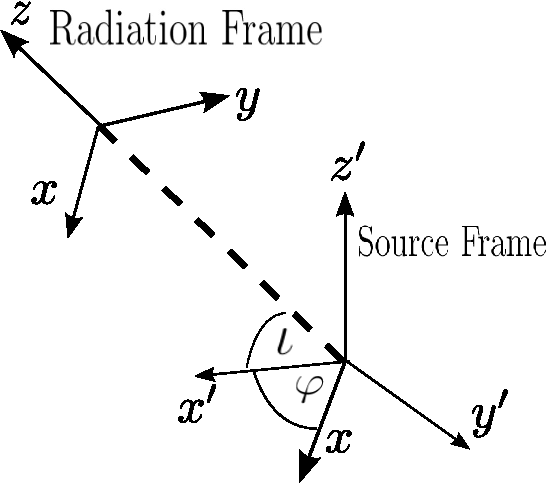
\includegraphics[width=0.5\linewidth]{Images/skyangles2.pdf}
  \caption[The angles that describe the relationship between the source
and radiation frames.]{\label{fig:intro_det_source}
A diagram that shows the geometric conversion from a ``radiation frame'' ($x-y$) to a ``source frame'' ($x'-y'$). Figure originally published in \cite{Mckechan:2010}.}
\end{figure}
%
\bea \left( \begin{array}{c} x' \\ y' \\ z' \end{array} \right)=
\left( \begin{array}{ccc}
\cos \varphi & - \sin \varphi & 0 \\
\sin \varphi & \cos \varphi & 0 \\
0 & 0 & 1
\end{array} \right)
\left( \begin{array}{ccc}
1 & 0 & 0 \\
0 & \cos \iota & -\sin \iota \\
0 & \sin \iota & \cos \iota
\end{array} \right)
\left( \begin{array}{c} x \\ y \\ z \end{array} \right)
\eea
%
\be \left( \begin{array}{c} x' \\ y' \\ z' \end{array} \right)=
R
\left( \begin{array}{c} x \\ y \\ z \end{array} \right) \ee
%
The new ``source'' quadrupole moment will then be defined as:
%
\begin{equation}
M_{ij}' = {\rm \bf R}^T(\theta, \phi)~M_{ij}~{\rm \bf R}(\theta, \phi)
\end{equation}
%
The equation for $h_{ij}$ is then written as ~\cite{Maggiore:gw, 1999physics8041C}
%
\be \label{eq:intro_h_dom}
h_{ij}^{TT}(t) = \frac{2}{D} \ddot{M}_{ij} \left(t - D\right). \ee
%
and the $h_+$ and $h_{\cross}$ components are given by
%
\be h_{+} = \frac{1}{D} \left(\ddot{M}_{11} - \ddot{M}_{22}\right) \ee
\be h_{\cross} = \frac{2}{D} \ddot{M}_{12}. \ee
%
Rotating the ``source'' quadrupole moment into the ``radiation frame'' we can write the
$h_+$ and $h_{\cross}$ components of the gravitational radiation as function of components of ``source'' moments $\ddot{M}'_{ij}$:
%
\begin{subequations}
\label{eq:gwemissionmain}
 \begin{align}
h_+ = \frac{1}{D} &\biggl[\ddot{M}'_{11}\left(\cos^2\varphi - \sin^2\varphi
\cos^2\iota\right) \nonumber \\ \nonumber &+ \ddot{M}'_{22}
\left(\sin^2\varphi - \cos^2 \varphi \cos^2\iota
\right) \\&- \ddot{M}'_{33}\sin^2 \iota - \ddot{M}'_{12}\sin 2\varphi
\left(1+ \cos^2 \nonumber
\theta\right) \\ &+ \ddot{M}'_{13} \sin\varphi \sin 2\iota + \ddot{M}'_{23}
\cos \varphi
\sin2\iota \biggr]
\label{eq:gwemission006}\\
h_{\cross} = \frac{1}{D} &\biggl[ \left(\ddot{M}'_{11} - \ddot{M}'_{22}\right)
\sin2\varphi \cos\iota + 2\ddot{M}'_{12}\cos2\varphi\cos\iota \nonumber
 \\ &- 2\ddot{M}'_{13}\cos
\varphi\sin\iota + 2\ddot{M}'_{23}\sin\varphi\sin\iota\biggr] .
\label{eq:gwemission007}
\end{align}
\end{subequations}
While higher order multipole moments of the mass distribution can contribute to the radiation, for most systems the quadrupole will dominate. Further, the mass monopole and dipole moment will not contribute any gravitational waves. Thus, such events as a spherically symmetric gravitational collapse and axially symmetric rotation do not emit any gravitational radiation. On the other hand, a rotating dumbbell is an excellent emitter of gravitational waves, making binary systems potentially amongst the brightest emitters of gravitational waves in the Universe.

\section{Gravitational waves from a compact binary coalescence} 
Two compact stars (two neutron stars, two black holes or a neutron star and a black hole) orbit each other in a 
close orbit and due to the very strong gravitational field produced by this system, gravitational waves are emitted. By emitting gravitational waves, the system loses energy and angular momentum hence the separation between the objects lessens with every orbit. The closer the stars get to each other, the more orbital energy is converted into gravitational waves, hence, the stronger the gravitational wave emission is. Eventually, the two compact objects will merge. This is called a compact binary coalescence, or CBC event. This system can be easily modelled analytically, in a Newtonian approximation, as described below. Using this approximation, we will derive the gravitational radiation waveform emitted from a \ac{CBC} event with point--like components (masses). This derivation will closely follow the formalism and workflow previously presented in \cite{Maggiore:gw,ian}, and we invite the reader to consult these references (and references therein) for a more detailed explanation.

\subsection{Compact binary coalescence parameters}

Let us consider now a Keplerian binary system far away from an observer $O$. It will be useful to begin by enumerating the physical parameters that are used in defining a \ac{CBC} system. These definitions will be used throughout all of the next chapters. A non--spin components \ac{CBC} on circular orbits can be completely described by nine physical parameters; these are the following:
%
\begin{itemize}
 \item The two masses, ($m_1$, $m_2$),
 \item The coalescence time of the signal at an observer at Earth, $t_c$,
 \item The sky location of the source -- two angles, ($\theta$,$\phi$),
 \item The distance to the source, $D$,
 \item The inclination angle, $\iota$,
 \item The coalescence phase, $\Psi_c$,
 \item The polarization phase, $\psi$.
\end{itemize}
%
The masses of the system are often combined in a number of different ways, these are
given by
%
\begin{itemize}
 \item The total mass, $M$ = $m_1$ + $m_2$,
 \item The chirp mass, $\mathcal{M} = \frac{(m_1 m_2)^{3/5}}{(m_1 + m_2)^{1/5}}$,
 \item The symmetric mass ratio, $\eta = \frac{m_1 m_2}{(m_1 + m_2)^2}$,
 \item The reduced mass, $\mu = \frac{m_1 m_2}{m_1 + m_2}$.
\end{itemize}
%
We also use the following binary orbit--related definitions;
%
\begin{itemize}
 \item The \textit{orbital} phase of the system, $\Psi$,
 \item The phase \textit{of the dominant mode of the emitted signal}, $\Phi = 2\Psi$,
 \item The \textit{orbital} angular frequency, $\omega$,
 \item The frequency \textit{of the emitted GW signal}, $f_{gw}$,
 \item The orbital radius of the system, $r$.
\end{itemize}

\subsection{Time evolution of the system}

Let's consider now equation (\ref{inertia}) for which we would like to find a solution only for the dominant order terms in $\lvert \mathbf{r}_1 - \mathbf{r}_2\rvert$. We consider such a system of two inspiralling compact objects, orbiting each other around the common center of mass (CM). The orbit is considered plane circular and obeying the classical Keplerian laws for celestial mechanics. The system can be considered in quasi--equilibrium  at any given time $t$ much smaller than the coalescence time if
%
\begin{equation}
\frac {{\rm d} \omega(t)}{{\rm d}t} \ll \omega^2(t)
\end{equation}
%
The separation vector ${\bf r}=(r_i(t))$ between the binary components will decrease gradually and reach zero at merger. In plane, Cartesian coordinates, the system is described by the position coordinates with respect to the center of mass:
%
\begin{equation}
r_1(t) = |{\bf r}| \cos (\omega t+ \phi_0), \hspace{10mm}
r_2(t) = |{\bf r}| \sin (\omega t+ \phi_0), \hspace{10mm}
r_3(t)=0
\end{equation}
%
In the center of mass of the system the moment of inertia (the second mass moment) is:
%
\begin{equation}
M^{ij} = \mu~r^i(t)~r^j(t)
\end{equation}
%
where $\mu=m_1m_2/(m_1+m_2)$ is the reduced mass.
If we differentiate this with respect to time twice we obtain
%
\begin{eqnarray}
\label{eq:mdoudbledot}
\ddot{M}_{11} &=& -\ddot{M}_{22} = 2\mu r^2\omega^2 \cos\left(2\int_0^{t}\omega(t') dt'\right) \\
\ddot{M}_{12} &=& - 2\mu r^2\omega^2 \sin\left(2\int_0^{t}\omega(t') dt'\right) \\
\ddot{M}_{13} &=& \ddot{M}_{23} = \ddot{M}_{33} = 0,
\end{eqnarray} 
%
where we assume that $r \omega \gg \dot{r}$. When this is not true the system is
not in a true circular motion.

We will write the solution to equation (\ref{inertia}) given by equations (\ref{eq:gwemission006}) and (\ref{eq:gwemission007}) in a geocentric reference frame:

\begin{subequations}
\begin{align}
h_{+} &= \frac{2\mu\omega^2 r^2}{D} \left( 1 + \cos^2 \iota \right)
\cos\left(\Phi(t) + 2\varphi\right) \\
h_{\cross} &= -\frac{2\mu \omega^2 r^2}{D} 2\cos \iota \sin
\left(\Phi(t)+ 2\varphi\right),
\end{align}
\end{subequations}
%
where the gravitational wave phase is defined as
%
\be \label{eq:cbc_grav_phase} \Phi(t) = 2\int_0^{t}\omega(t') dt'. \ee
%
Expanding $r$ in terms of $\omega$ by using Kepler's third law of planetary motion:
%
\be \omega^2 = \frac{m_1 + m_2}{r^3}. \ee
%
we can then write $h_+$ and $h_{\cross}$ as
%
\begin{subequations}
\label{eq:cbc_hplus_cross}
\begin{align}
h_{+}(t) &= \frac{2}{D}\mathcal{M}^{5/3}\omega(t)^{2/3}\left( 1 + \cos^2 \iota \right)
\cos\left(\Phi(t)+ 2\varphi\right) \\
h_{\cross}(t) &= -\frac{2}{D}\mathcal{M}^{5/3}\omega(t)^{2/3} (2\cos \iota) \sin \left(
\Phi(t)+ 2\varphi\right).
\end{align}
\end{subequations}

\subsection{Energy loss in the system}
\label{sec:cbc_energyloss}

Due to emission of \ac{GW}, the orbital angular velocity $\omega$ will increase with time. Expressing $\omega = \omega(t)$, we can find a measure of the rate at which the system radiates \ac{GW} energy. The total radiated energy in time can be obtained by integrating the time--dependent flux, then the power radiated by a gravitational wave is given as \cite{Maggiore:gw,ian}
%
\be \frac{\mathrm{d}E}{\mathrm{d}t} = \frac{1}{16 \pi} \int d\Omega \langle \dot{h}_+^2 +
\dot{h}_{\cross}^2 \rangle. \ee
%
Equation (\ref{eq:intro_rad_power}) gives us a general formula for the energy loss, to leading order:
%
\be
\label{eq:intro_rad_power}
\frac{\mathrm{d}E}{\mathrm{d}t} = \frac{1}{5} \langle \dddot{M}'_{ij} \dddot{M}'^{ij}
- \frac{1}{3}(\delta^{kl}\dddot{M}'_{kl})^2\rangle. \ee
%
To obtain the third differential of the moment of inertia, we will perform a further differentiation on equation (\ref{eq:mdoudbledot}):
%
\begin{subequations}
\label{eq:mtripledot}
\begin{align}
\dddot{M}_{11} &= -\dddot{M}_{22} = -4\mu r^2\omega^3 \sin\left(2\int_0^{t}\omega(t') dt'\right) \\
\dddot{M}_{12} &= - 4\mu r^2\omega^3 \cos\left(2\int_0^{t}\omega(t') dt'\right) \\
\dddot{M}_{13} &= \dddot{M}_{23} = \dddot{M}_{33} = 0.
\end{align}
\end{subequations}
%
The power radiated by the system is then calculated by inserting equation (\ref{eq:mtripledot}) into (\ref{eq:intro_rad_power}). Using the assumption that for circular orbits $\langle \sin^2 \Phi(t) \rangle = \langle \cos^2 \Phi(t) \rangle = \frac{1}{2}$ we get
%
\be \label{eq:cbcwav_power} P = - \frac{\mathrm{d} E_{orbit}}{\mathrm{d}t} = \frac{32}{5}\left(\mathcal{M} \omega
\right)^{10/3}, \ee
%
which is the total radiated power of the system, to dominant order. The emitted power is proportional to the chirp mass to an exponent $\approx 3$: the heavier the system, the more radiated power. Also, emitted power is proportional to the orbital frequency to an exponent $\approx 3$: the closer the binary components, the higher the frequency thus the more radiated power.

\subsection{Phase evolution of the system}
\label{sec:cbc_phaseevol}

It follows from equation (\ref{eq:cbcwav_power}) that if we write the expression for the total energy of the system, we can compute the time--variance of the orbital angular velocity. Consider the total energy of the system as the sum of kinetic and gravitational potential contributions:
%
\begin{align} \label{eq:cbcwav_etot}
E_{orbit} &= -\frac{m_1 m_2}{r} + \frac{m_1 m_2}{2r} = -\frac{m_1 m_2}{2r} \nonumber \\
&= - \left( \mathcal{M}^5 \omega^2/8\right)^{1/3},
\end{align}
%
differentiate this with respect to time and insert it into equation (\ref{eq:cbcwav_power}) to get
%
\be \frac{32}{5}
\left(\mathcal{M} \omega\right)^{10/3}
=  \mathcal{M}^{5/3} \frac{1}{3}
 \omega^{-1/3} \dot{\omega}. \ee
%
This formula can be rearranged to give the change in orbital angular velocity with
respect to time, $\dot{\omega}$, as
%
\be \dot{\omega} = \frac{96}{5} \mathcal{M}
^{5/3} \omega^{11/3}. \ee
%
The orbital angular frequency can then be expressed as a function of time,
by integrating this equation, provided initial conditions, from a limit time $t_0$ with an initial orbital
frequency $\omega_0$
%
\be \omega(t) = \left(-\frac{256}{5} \mathcal{M}
^{5/3}\left( t - t_0 \right) + \omega_0^{-8/3} \right)^{-3/8}. \ee
%
We can see that  for a time $t \rightarrow t_0$ $\omega$ will diverge to infinity. At this limit, the two bodies will not be in circular motion anymore and will start plunging towards each other. But this time is finite and  for simplification let us take this as our limit time, which we will call $t_{c}$, time of coalescence. This choice serves to set $\omega_0^{-8/3}$ to zero. If we introduce a time variable change to
%
\be \tau \equiv t - t_{c} \ee
%
$\omega$ can be re--expressed in terms of $\tau$ as
%
\be \label{eq:omegatau}
\omega(\tau) = \frac{1}{8}\left(\frac{\tau}{5}\right)^{-3/8}
\mathcal{M}^{-5/8},  \ee
%
and in SI units:
%
\be \label{eq:omegatauSI}
\omega(\tau) = \frac{1}{4}\left(\frac{\tau}{5}\right)^{-3/8}
\left({\frac{G\mathcal{M}}{c^3}}\right)^{-5/8},  \ee
%

Now $\Phi(t)$ can be evaluated by combining equations (\ref{eq:cbc_grav_phase}) and (\ref{eq:omegatau})
%
\begin{subequations}
\begin{align}
\Phi(\tau) &= 2\int_{t_{c}}^{\tau}\frac{1}{8}\left(\frac{\tau'}{5}\right)^{-3/8}
\mathcal{M}^{-5/8} d\tau' \\
\label{eq:cbc_phase_tau}
\Phi(\tau) &= 2 \left(\frac{\tau}{5 \mathcal{M}}\right)^{5/8}
 - 2 \left(\frac{t_{c}}{5 \mathcal{M}}\right)^{5/8}.
\end{align}
\end{subequations}
%
Finally, this allows $h_+$ and $h_{\cross}$ to be evaluated in the time domain by combining equations
(\ref{eq:cbc_hplus_cross}), (\ref{eq:omegatau}) and (\ref{eq:cbc_phase_tau}).

\subsection{Frequency domain waveforms}
\label{sec:cbc_freqdom}

It is often useful in gravitational wave searches to express $h_+$ and $h_{\cross}$ in the frequency
domain. This can be done by performing a Fourier transform on $h_+$ and $h_{\cross}$.

Firstly, to express $\tau$ as a function of frequency, equation (\ref{eq:omegatau}) is rearranged, remembering that $\omega = \pi f$, to get
%
\be \label{eq:taufreq}
\tau(f) = \frac{5}{256}(\pi f)^{-8/3} \mathcal{M}^{-5/3}.
\ee
%
Inserting this into equation (\ref{eq:cbc_phase_tau}) gives
%
\be \Phi(f) = \frac{1}{16} f^{-5/3} \mathcal{M}^{-5/3} - 2 \left(\frac{t_{c}}{5 \mathcal{M}}\right)^{5/8}
\label{phasefivethirds}
\ee
%
and the time domain waveforms can be written in terms of the frequency
%
\begin{subequations}
\label{eq:cbc_hp_hc_freq}
\begin{align}
h_{+}(\tau) &= \frac{2}{D} \mathcal{M}^{5/3}
\left( \pi f(\tau) \right)^{2/3}
\left( 1 + \cos^2 \iota \right)
\cos \left(
\Phi(f(\tau)) + 2\varphi\right) \\
h_{\cross}(\tau) &= -\frac{2}{D} \mathcal{M}^{5/3}
\left( \pi f(\tau) \right)^{2/3}
(2\cos \iota)  \sin \left(
\Phi(f(\tau)) + 2\varphi\right).
\end{align}
\end{subequations}
%
To convert this into the Fourier domain, $\tilde{h}_+$ and $\tilde{h}_{\cross}$,
a Fourier transform could be performed on the time domain waveforms. Performing a Fourier transform numerically may often prove to be computationally expensive, hence it is desirable to have an analytical formula for the frequency domain waveforms. This can be obtained by using the \emph{stationary phase approximation} (SPA). This approximation is used in cases of rapidly--varying phase terms. Using \cite{Bro04}, we will define the stationary phase approximation: given a harmonic function with a time--varying amplitude, e.g.,
%
\be F(t) = A(t) \cos(\phi(t)), \ee
%
where
%
\be \frac{1}{A} \frac{\mathrm{d} A}{\mathrm{d}t} \ll \frac{\mathrm{d} \phi}{\mathrm{d}t} \ee
%
at all times $t$; for a GW emitted by a CBC, the phase change over time is much larger than the relative amplitude change over time. The Fourier transform of $F(t)$ can be approximated as
%
\be \tilde{F}(f) \approx \frac{1}{2} A(f) \left(\frac{\mathrm{d}f}{\mathrm{d}t}\right)^{1/2}
\exp\left[ -i \left(2 \pi f t' - \phi(f) - \frac{\pi}{4}\right)\right],
\ee
%
where $t'$ is defined as the time at which
%
\be \left( \frac{\mathrm{d} \phi(t)}{\mathrm{d}t} \right)_{t=t'}= \pi f \ee
%
The stationary phase approximation can be applied to $h_+$ and $h_{\cross}$ to give analytical formulae for the frequency domain waveforms. To evaluate these frequency domain waveforms we first need to evaluate $\frac{\mathrm{d}f}{\mathrm{d}t}$. Using equation (\ref{eq:omegatau}) and $\omega = \pi f$ we get
%
\be \frac{\mathrm{d}f}{\mathrm{d}t} = -\frac{\mathrm{d}f}{\mathrm{d}\tau} = \frac{3}{320 \pi} \left(\frac{\tau}{5}\right)^{-11/8}
\mathcal{M}^{-5/8}, \ee
%
this can be expressed in terms of frequency by substituting equation (\ref{eq:taufreq})
%
\be \frac{\mathrm{d}f}{\mathrm{d}t} = \frac{96}{5} \pi^{8/3} f^{11/3} \mathcal{M}^{5/3}. \ee
%
The stationary phase frequency domain waveforms can then be written, to the leading order, as
%
\begin{subequations}
\label{eq:cbc_hp_hc_spa}
\begin{align}
\tilde{h}_{+}(f) &= \frac{1}{D} \left(\frac{5}{96}\right)^{1/2}
\mathcal{M}^{5/6} \pi^{-2/3} f^{-7/6}
\left( 1 + \cos^2 \iota \right)
\exp \left[ i \left(2\pi f t' -
\Phi(f) - \frac{\pi}{4} - 2\varphi\right)\right] \\
\tilde{h}_{\cross}(f) &= -\frac{1}{D} \left(\frac{5}{96}\right)^{1/2}
\mathcal{M}^{5/6} \pi^{-2/3} f^{-7/6}
(2\cos \iota)
\exp \left[ i \left(2\pi f t' -
\Phi(f) + \frac{\pi}{4} - 2\varphi\right)\right].
\end{align}
\end{subequations}
%
Equations (\ref{eq:cbc_hplus_cross}), (\ref{eq:omegatau}), (\ref{eq:cbc_phase_tau}) and (\ref{eq:cbc_hp_hc_spa}) describe the evolution of the \ac{GW} waveforms from a \ac{CBC} event to first order in both time and frequency domains.

This set of calculations have been derived using a Newtonian mechanics approximation, i.e. considering circular orbits. Introducing relativistic corrections is beyond the scope of this thesis. The Post--Newtonian formalism allows the phase evolution of the binary system to be predicted with much higher accuracy than the approximate derivation given here \cite{Buonanno:2009zt,Bliving}. The Post--Newtonian expansion uses perturbative techniques to expand the phase of the system to higher order terms. Generally the expansion is performed around $(\pi M f)^{1/3}$.

In equation (\ref{phasefivethirds}) we have shown that the leading order term in time domain phase evolution is a multiple of $f^{-5/3}$. The next term, the ``1 PN'' term enters at $f^{-3/3}$, the ``1.5 PN'' term enters
at $f^{-2/3}$ and so on (there is no 0.5 PN term proportional to $f^{-4/3}$). Current non--spinning Post--Newtonian expansions generally include all terms up to 3.5 PN order \cite{Buonanno:2009zt}.

In addition to higher--order phase terms, there are also higher--order amplitude terms. These higher--order amplitude terms arise from the octopole (and consequently higher) moments and therefore the phase of these terms is not necessarily twice the orbital phase. A study of these higher order amplitude terms and how they might affect our ability to detect \ac{CBC} systems can be found in \cite{Mckechan:2010}, but the importance of these higher order amplitude terms is much less than the higher order frequency terms.

Another remark we have to make is that, in general relativistic geometry, there is a minimal radius beyond which circular orbits are no longer possible -- the Innermost Stable Circular Orbit (ISCO). This is defined in Schwarzschild geometry for a point mass around a black hole

\be r_{\mathrm{ISCO}} \equiv \frac{6GM}{c^2} \ee

We may extend this definition to a binary system of compact stars -- this will, of course, be an approximation from the rigorous definition of ISCO. In such a system, the ISCO radius defines the limit between weak--field and strong--field, and using this, the maximum frequency at which the binary is still in a quasi--Keplerian motion is
%
\be f_{\mathrm{ISCO}} = \frac{c^3}{6 \sqrt{6} \pi GM} \ee
%
With this in mind we see that the inspiral phase of a system of binary neutron stars (NS--NS) each with a mass of $m_1 = m_2 \approx 1.4 M_{\odot}$ will end at a frequency of $f \sim 1600$~Hz. For a stellar mass binary black hole system this frequency will reduce to  $f \sim 100-200$~Hz and for a supermassive binary black hole system it will be in the mHz range. These values are very important when building GW detectors: depending on the detectors' construction and subsequent operational frequency window, different GW detectors are sensitive to different GW sources.


\section{Gravitational Wave Detectors -- Theoretical Aspects}

\subsection{A simplified laser interferometer}

The most widely used and altogether the largest and most sensitive type of \ac{GW} detector uses laser light interferometry as functional principle. A simplified schematic of a Michelson laser interferometry GW detector is pictured in Figure ~\ref{ligo_optics}.

\begin{figure}[ht]
\centering
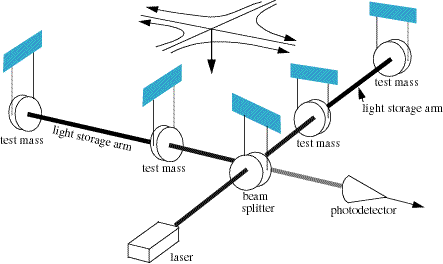
\includegraphics[scale=0.70]{Images/interferometer.png}
\caption{Optical set--up schematics for a \ac{GW} interferometer. Image initially published and adapted from \cite{Abadie:2010px}}
\label{ligo_optics}
\end{figure}

It consists of two arms oriented at a $90^\circ$ angle with laser beams running along the length of the arms. The laser light is emitted at the center of the ``L'' shape and split using a beam splitter, the light then travels along each of the arms, is reflected by mirrors at the end of each arm, passes back down along the arms and is recombined
at the initial starting point. A plane gravitational wave incident to the plane of the detector affects the two ``L'' arms differently, by simultaneously lengthening one while shortening the other. By measuring this differential effect one can measure the \ac{GW} strain. As the path length for the light to travel down the arms varies, the laser light being recombined will have a variable phase difference and thus by observing the interference pattern we can measure the change in path length between the two arms, created by the \ac{GW} passage.  We will briefly describe what are the physical principles based on which such an interferometer will operate. These are described in detail in \cite{Saulson:1994} and we will summarize the main concepts. The electric field of the input laser light is given by
%
\begin{equation} 
|{\bf E}_{\rm in}| = |{\bf E}_0| \mathrm{e}^{2 \pi ift - i \mathbf{k} \cdot \mathbf{x}}
\end{equation}
%
where $f$ is the frequency of the light and $\mathbf{k}$ is the wave vector. $E_0$
denotes the amplitude of the laser light. Consider the beam splitter to be at $\mathbf{x} = 0$.
The beam splitter will send equal power along each arm so that we can describe the light,
transmitted by the beam splitter and travelling down the $x, y$ arms by the electric fields $|{\bf E}_{\rm in}| = (E_{x},~E_{y})$:
%
\begin{equation} 
E_{x} = \frac{E_0}{\sqrt{2}} \mathrm{e}^{2 \pi ift - i \lvert \mathbf{k} \rvert x}
\end{equation}
%
\begin{equation} 
E_{y} = i \frac{E_0}{\sqrt{2}} \mathrm{e}^{2 \pi ift - i \lvert \mathbf{k} \rvert y}
\end{equation}
%
where $T = 1/\sqrt{2}$ is the transmission coefficient and $R = i/\sqrt{2}$ the reflection coefficient.

After the light is reflected at the end of each arm, the electric fields will be given by:
%
\begin{eqnarray}
 E_{x} = \frac{E_0}{\sqrt{2}} \mathrm{e}^{2 \pi if t - i 2 k L_x} \\
 E_{y} = i \frac{E_0}{\sqrt{2}} \mathrm{e}^{2 \pi if t - i 2 k L_y},
\end{eqnarray}
%
where $L_x$ and $L_y$ denote the path length along the $x$ and $y$ arms respectively. After consecutive reflexions and transmissions the light beams are combined at the photodetector and its electric field is expressed as:
%
\be
  E_{\rm out} = i \frac{E_0}{2} \left( \mathrm{e}^{2 \pi if t - 2 ik L_x} + \mathrm{e}^{2 \pi if t - 2 i k L_y}\right).
\ee
%
and can be re--written as:
%
\be
  E_{\rm out} = i E_0 \mathrm{e}^{2 \pi ift - k (L_x + L_y)}
\cos\left(k (L_x - L_y)\right).
\ee
%
The interferometer is locked to the dark fringe, i.e. in the case of equal path lengths $L_x = L_y = L$ the resultant power at the detecting port should be zero. Since the power of a beam of light is proportional to the squared electric field amplitude, we can see that in case of a variation in path length the dark port will have residual power of the order
%
\be
  \Delta P_{\rm out} \propto 1 + \cos\left(2 k (L_x - L_y)\right).
\ee
%
Thus any variation of the relative path length $\Delta L = L_x - L_y$ of the arms would cause a variation in the
power incident on the photodetector.

In this section we have only given a very simplistic description of
how an interferometer works. For a
more comprehensive description of the operation of modern interferometers and
the methods used to increase sensitivity see \cite{Saulson:1994,Maggiore:gw}.

\subsection{Response of an interferometer to a gravitational wave}
\label{section:interferometerresponse}

\subsubsection{The effect of a \ac{GW} at the detector}
In order to illustrate the effect a \ac{GW} would have on the local geometry of a detector we will first use the example of test particles on a ring. Consider a circular string of test masses subject to the passage of a plane monochromatic gravitational wave $h(t)=(h_+, h_{\cross})= (A_+\cos\left(\omega t - \omega z + \phi_0 \right), A_{\cross}\cos\left(\omega t - \omega z + \phi_0 \right))$ -- the wave is fully described by the two polarizations $+,\cross$. We can write the proper distance between any two given points as the interval $ds$:
%
\begin{equation}
ds^2 = g_{\mu\nu}dx^{\mu}dx^{\nu} = (\eta_{\mu\nu} + h_{\mu\nu})dx^{\mu}dx^{\nu}
\end{equation}
%
and expressing the \ac{GW} in terms of the two polarizations
%
\begin{align}
ds^2 = &-c^2dt^2 + dz^2 + \left( 1 + A_+\cos\left(\omega t - \omega z + \phi_0 \right)\right)
dx^2 \\
&+ \left( 1 - A_+\cos\left(\omega t - \omega z + \phi_0 \right)\right)dy^2 +
2A_{\cross}\cos\left(\omega t - \omega z + \phi_0 \right)dxdy.  \nonumber
\label{hONdetector}
\end{align}
%
If we then consider two particles at positions $(x_1,y_1,0)$ and $(x_2,y_2,0)$ the proper distance between them at some arbitrary time $t$ would be given by
%
\begin{align}
ds^2 =& \left( 1 + A_+\cos\left(\omega t - \omega z \right)
\right)\left(x_1-x_2\right)^2 \nonumber
+ \left( 1 - A_+\cos\left(\omega t - \omega z \right)\right)\left(y_1-y_2\right)^2
\\ &+ 2A_{\cross}\cos\left(\omega t - \omega z \right)
\left(x_1-x_2\right)\left(y_1-y_2\right)
\end{align}
%
This quantity is time dependent. Take for example the simplification that $y_2 - y_1 = 0$ this equation would become
%
\be ds^2 = \left( 1 + A_+\cos\left(\omega t - \omega z \right)
\right)\left(x_1-x_2\right)^2, \ee
%
and the proper distance is
%
\be ds \approx \left(1 + \frac{1}{2}A_+\cos\left(\omega t - \omega z \right)
\right)
\left(x_1 - x_2\right), \ee
%
where we have used the fact that in the weak field limit $A_+ \ll 1$.

The effect of the $+$ and $\times$ polarizations is shown in Figure \ref{massesGW}. The gravitational wave, when passing through the interferometer, will alter the lengths of the light arms (paths) just as the particles separation is altered in Figure \ref{massesGW}.

\begin{figure}[ht]
%\begin{minipage}[b]{0.5\linewidth}
\centering
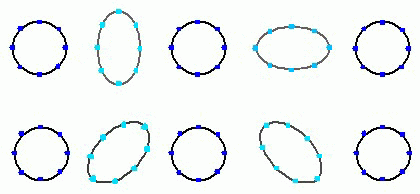
\includegraphics[scale=0.65]{Images/massesGW.png}
%\caption{Effect of passage of $+$ polarization. Image reproduced from \cite{ian}}
%\label{fig:massesplus}
%\end{minipage}
%\hspace{0.5cm}
%\begin{minipage}[b]{0.5\linewidth}
%\centering
%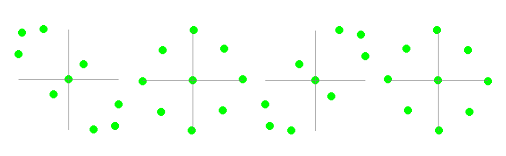
\includegraphics[scale=0.35]{Images/cross.png}
\caption{Effect of passage of $+$ polarization (top row) and effect of passage of $\times$ polarization (bottom row) through a ring of particles: the effect is of squeezing and extending along different axes for the two GW polarizations.}
\label{massesGW}
%\end{minipage}
\end{figure}

When a gravitational wave passes through the interferometer, the space--time in the local area is altered. Depending on the source of the wave and its polarization, this results in an effective change in the length of one or both of the ``L'' arms. Consider a gravitational wave detector with two equal length arms pointing along the $x$ and $y$ directions and suppose an incident gravitational wave propagating along the $z$ direction towards the detector. Knowing that light travels along null geodesics hence $\mathrm{d}s^2=0$, we can estimate the change in light time along each of the detector's arms. For the $x,~y$ axes
%
\be 0 = -c^2\mathrm{d}t^2 + (1 + h_+(t)) \mathrm{d}x^2 \ee
%
Integrating, the light time will be along the $x$ axis
%
\be \Delta t_x = t_x - t_0 = \frac{1}{c}\int_0^{L_0} \sqrt{1 + h_+} \mathrm{d}x \approx \frac{L_0}{c} + \frac{1}{2c}\int_0^{L_0} h_+ \mathrm{d}x \ee
%
where $L_0$ is the length of the arm when no gravitational wave is incident on the detector and we have ignored terms that are second order in $h_+$. The integral on the right of this equation is easily evaluated if we assume that
$h_+$ does not vary significantly during travel along the arm, therefore taken as constant. This is a fair assumption for the realistic case of an interferometer with 4km arms and a gravitational wave with 100Hz frequency. The light travel time to travel up the $x$ arm is then given by
%
\be c \Delta t_x \equiv L_x = L_0 ( 1 + h_+ ) \ee
%
Similarly the light travel time down the arm is evaluated in the same way and has the same value. The difference in the light travel time to go up each arm and back to the beam splitter is then given by
%
\be \label{eq:intro_dt_simple}
c \Delta t = c(\Delta t_x - \Delta t_y) \equiv L_x - L_y =  L_0 h \ee
%
\be \label{varh_L} h = \frac{\Delta L}{L_0} = \frac{L_x - L_y}{L_0} \ee
%
Therefore as $h$ varies, the relative length of the two arms
will also vary. This will then cause variations in the power observed at the photodetector,
allowing us to directly observe the variation in the gravitational field.

There is, however, a significant difference between this simple explanation and an actual gravitational wave interferometer designed to detect gravitational radiation with amplitudes of order $h \sim 10^{-22}$. To achieve this level of sensitivity the operation of gravitational wave interferometers is much more complex than the description here. For example, Fabry--Perot cavities are used to increase the effective path length of the laser light and allow for multiple reflexions of the beams before recombination at the photodetector (an optical cavity or resonator is an arrangement of mirrors that forms a standing wave cavity for EM waves). Power recycling techniques and high powered lasers are used to maximize the power coming out of the beam splitter. A much more comprehensive description of the operation of gravitational wave interferometers and the difficulties they have to overcome can be found in \cite{Saulson:1994,Maggiore:gw}.

\subsubsection{Detector antenna pattern functions}
Gravitational wave detectors, like many other astronomical observatories, have a limited sensitivity to source detection, depending on the location and the properties of the source. They can be described, analogously to radio antennae, by expressing their sensitivity in terms of \emph{antenna factors}.

Consider again the $x-y$ plane of the detector with its two arms along $x$--axis and $y$--axis respectively. We will call this plane the \emph{detector frame}. Consider now an incident gravitational wave $h = (h_+, ~h_{\cross})$ with its two polarizations parallel to a different plane $x'-y'$. We will call this plane the \emph{radiation frame}. This more general case when the radiation frame is not aligned with the detector frame can be easily solved by performing a series of rotations (just as we did above when transitioning from radiation frame to GW source frame). The angles relating the detector frame to the radiation frame are shown in Figure \ref{fig:intro_det_rad}. The angles $(\theta,\phi)$ give the sky location of the source relative to the detector frame. These two angles translate us to a frame in which the perpendicular $z'$ on the radiation plane points from the source to the detector. A further angle, the polarization phase, $\psi$, is needed to rotate the $x$ and $y$ axes of this frame into the radiation frame.
%
\begin{figure}[tp]
  \centering
  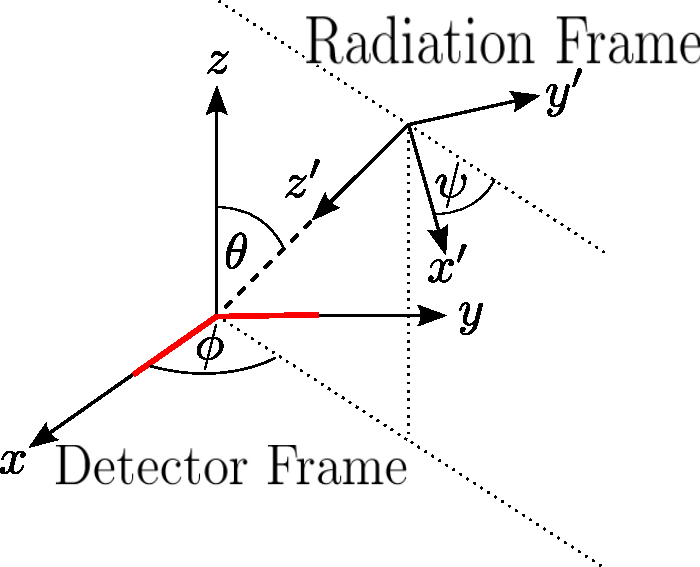
\includegraphics[width=0.5\linewidth]{Images/skyangles.pdf}
  \caption[The angles that describe the relationship between the detector
and radiation frames.]{\label{fig:intro_det_rad}
An illustration of the angles that describe the relationship between the detector
and radiation frames. Figure originally published in \cite{Mckechan:2010}.}
\end{figure}

The gravitational wave at the detector will be a linear combination of the two source polarizations
%
\be \label{eq:intro_hoft}
h(t) = F_+ h_+(t) + F_{\cross} h_{\cross}(t) \ee
%
In this expression $F_+$ and $F_{\cross}$ give the detector response to the $h_+$ and $h_{\cross}$ components respectively of the gravitational wave in the radiation frame. Explicitly these are given by \cite{Allen:2005fk}
%
\begin{subequations}
  \label{eq:fplus_fcross}
 \begin{align}
  F_+ (\theta,\phi,\psi) &= - \frac{1}{2}(1 + \cos^2\theta)\cos2\phi \cos2\psi
- \cos \theta \sin 2\phi \sin 2\psi \\
  F_{\cross} (\theta, \phi, \psi) &= \frac{1}{2}(1 + \cos^2\theta)\cos2\phi \sin2\psi
- \cos \theta \sin 2\phi \cos 2\psi
 \end{align}
\end{subequations}

The polarization angle of an incoming gravitational wave would generally be expected to be uncorrelated to its direction of arrival (polarization is related to orientations in the source). Then it is useful to characterize the  directional sensitivity of a detector by averaging over the polarization angle $\psi$. If we are interested in a single detector's response, it is always possible to align the polarization angle $\psi$ in the sky plane with that of the wave, so that the wave has pure $+$-polarization. Then the root mean square response function of the detector is 
%
\begin{equation}\label{eqn:rmsresponse}
F_{\mathrm{rms}} =  \left(\int F_+^2\mathrm{\ d}\psi \right)^{1/2}.
\end{equation}
%
The function $F_{\mathrm{rms}}$ is often simply called the \emph{antenna pattern} and for an interferometer, it is given by
%
\begin{equation}
F_{\mathrm{rms}} = \sqrt{F_+^2 + F_{\cross}^2} = \sqrt{ \frac{1}{4} \left ( 1 + \cos^2\theta \right)^2
\cos^2 2\phi + \cos^2\theta \sin^2 2\phi }
\end{equation}

\begin{figure}[ht!]
\centering
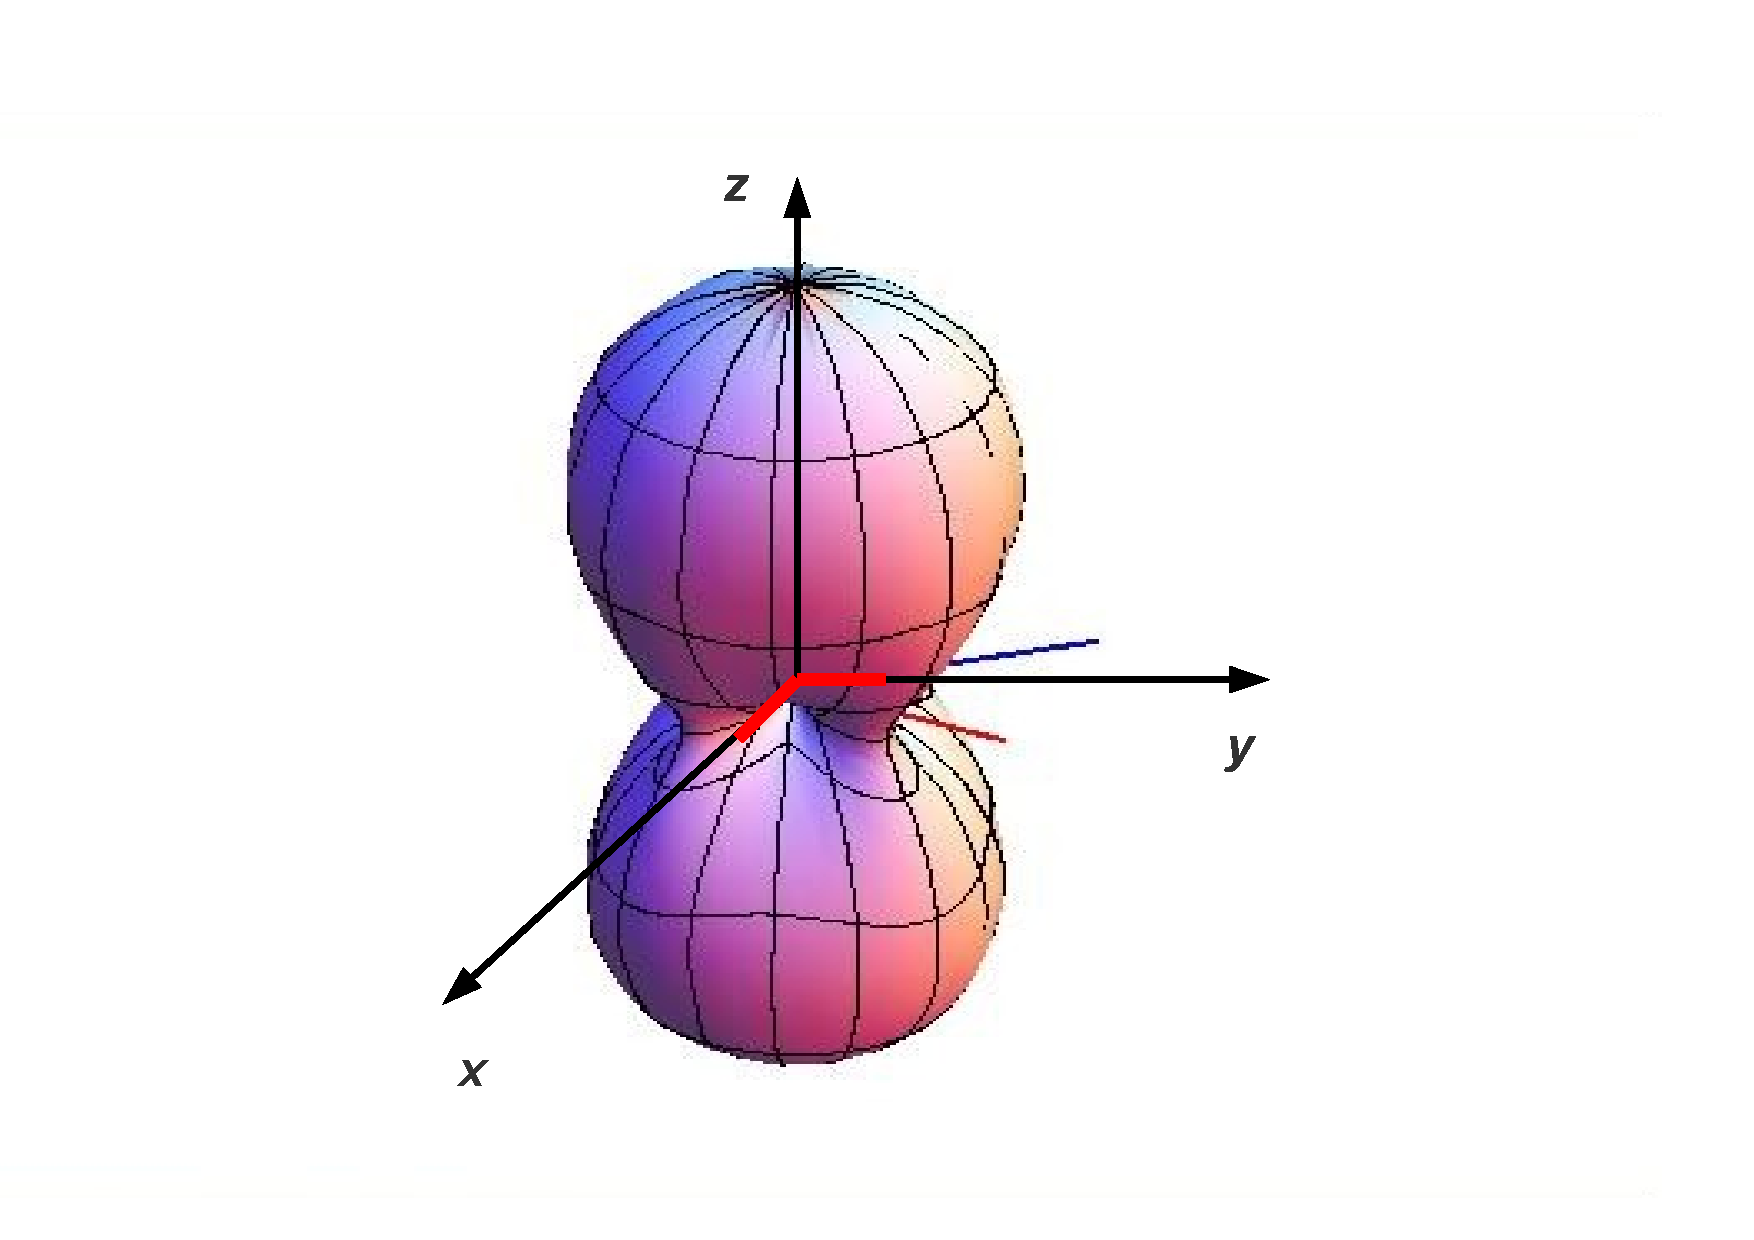
\includegraphics[scale=0.25]{Images/peanut.pdf}
\caption{A GW detector sensitivity to an unpolarized GW wave varies with the source direction -- here plotted the antenna response $F_+$ of an interferometric GW detector with the arms in the $x-y$ plane and oriented along the two axes. The response $F_+$ for waves coming from a certain direction is proportional to the distance to the point on the antenna pattern in that direction. This clearly shows the quadrupolar nature of the wave. Image reproduced and modified from ~\cite{Sathyaprakash:2009xs}}
\label{peanut}
\end{figure}

The Figure \ref{peanut} gives us an idea of how sensitive a single \ac{GW} detector can be to a gravitational wave with a certain polarization and incident from a certain direction on the sky: the response $F$ for waves coming from an arbitrary direction is proportional to the distance to the point on the antenna pattern in that direction; also this clearly shows the quadrupolar nature of the wave; a single detector has a limited capability of detecting waves with sources ``sub--optimally'' located - the ideal case would be a source directly overhead.   

\subsubsection{A CBC $h(\tau)$ at the detector}
We wish to calculate the strain that would be observed at a gravitational
wave detector due to the passage of a gravitational wave emitted by a \ac{CBC}.
To do this the expressions for $h_+(t)$ and $h_{\cross}(t)$ can be combined
with equations (\ref{eq:intro_hoft})
and (\ref{eq:fplus_fcross}) as follows:
%
\begin{subequations}
\begin{align}
h(\tau) =& F_+ h_+(\tau) + F_{\cross} h_{\cross}(\tau) \\
     =& \left(- \frac{1}{2}(1 + \cos^2\theta)\cos2\phi \cos2\psi
- \cos \theta \sin 2\phi \sin 2\psi\right) \nonumber \\
& \left(\frac{2}{D} \mathcal{M}^{5/3}
\left( \pi f(\tau) \right)^{2/3}
\left( 1 + \cos^2 \iota \right)
\cos \left(
\Phi(\tau)+ 2\varphi\right) \right) \nonumber \\
    &+ \left(\frac{1}{2}(1 + \cos^2\theta)\cos2\phi \sin2\psi
- \cos \theta \sin 2\phi \cos 2\psi\right) \nonumber \\
& \left(-\frac{2}{D} \mathcal{M}^{5/3}
\left( \pi f(\tau) \right)^{2/3}
(2\cos \iota) \sin \left(
\Phi(\tau)+ 2\varphi\right)\right). \nonumber
\end{align}
\end{subequations}
%
Re--writing these as harmonic functions with an amplitude and a phase term:
%
\be
\label{eq:h_amp_phase}
  h(\tau) = A(D,\iota,\theta,\psi,\phi)\mathcal{M}^{5/3}\left( f(\tau) \right)^{2/3} \cos\left(\Phi(\mathcal{M},\tau)
+ \Phi_0 (\iota,\varphi,\theta,\psi,\phi) \right),
\ee
%
where $A$ is a constant amplitude term and $\Phi_0$ a constant phase offset. Or equivalently
in the frequency domain as
%
\be
\label{eq:h_amp_phase_freq}
\tilde{h}(f) = \tilde{A}(D,\iota,\theta,\psi,\phi) \mathcal{M}^{5/6}f^{-7/6}
\exp\left[i\left(\Phi(\mathcal{M},f) + \tilde{\Phi}_0 (\iota,\varphi,\theta,\psi,\phi,t_c) \right)\right],
\ee
%
This shows that a single detector can only distinguish an amplitude and a phase for the incident \ac{GW} and it would not be possible to extract information on sky localization and distance to the source since amplitude and phase are degenerate. However, if more than one detector is used, the degeneracy can be broken and these parameters can be recovered. We note that if the phase evolution is evaluated to higher
order it will depend on $\eta$ as well as $\mathcal{M}$ and time/frequency.

\subsection{Gravitational radiation from a binary neutron star merger}
\label{sec:cbc_example}

It is useful to consider a practical example of a binary neutron star merger, using the theoretical derivations we have have done in the previous sections. Consider a compact binary neutron star inspiral, with both components approximated to point--like masses having typical neutron star masses of $m_1 = m_2 = 1.4M_{\odot}$. Let this system be located at a distance of $D=1~\mathrm{Mpc}$ and ideally directly over a detector hence $\theta=\phi=0$. Additionally, let it be ideally oriented such that $\iota = \varphi = \psi = 0$. The gravitational waveform at the detector, in such a case, would have the expression from equation (\ref{eq:h_amp_phase}) in SI units:

\begin{equation}
h(\tau) = \frac{1}{D} A(\iota,\theta,\psi,\phi) \mathcal{M}^{5/3}f^{2/3} \mathrm{e}^{i\left(\Phi(\mathcal{M},f) + \tilde{\Phi}_0 \right)}
\end{equation}
%
where

\be
A(\iota=0,\theta=0,\psi=0,\phi=0) = \frac{4 \pi^{2/3} \left( G \mathcal{M} \right)^{5/3}}{c^4}
\ee
%
and using equation (\ref{eq:omegatau}) we obtain the expression $h(\tau)$:

\begin{equation}
h(\tau) = \frac{1}{D} \left( \frac{G \mathcal{M}}{c^2} \right)^{5/4} \left( \frac{5}{c \tau} \right)^{1/4} \mathrm{e}^{i\left(\Phi(\mathcal{M},\tau) + \Phi_0 \right)}
\end{equation}
%
Plugging in the numbers for $\mathcal{M} = 1.21 ~M_{\odot}$ and $D=1~\mathrm{Mpc}$ we obtain an amplitude 
%
\be
A(\tau) \approx \frac{10^{-21}}{\tau^{1/4}}
\ee
%
The gravitational waveform that this system would produce in the detector is shown, in the time domain, in Figure \ref{chirpwaveT} and is the ``chirp--wave''. This also shows the order of magnitude of the strain we expect to detect from a binary neutron star coalescence at a reference distance $D=1~\mathrm{Mpc}$ and ideal orientation and localization, $h(\tau) \approx 10^{-21} / \tau^{1/4}$.

\begin{figure}[ht]
\centering
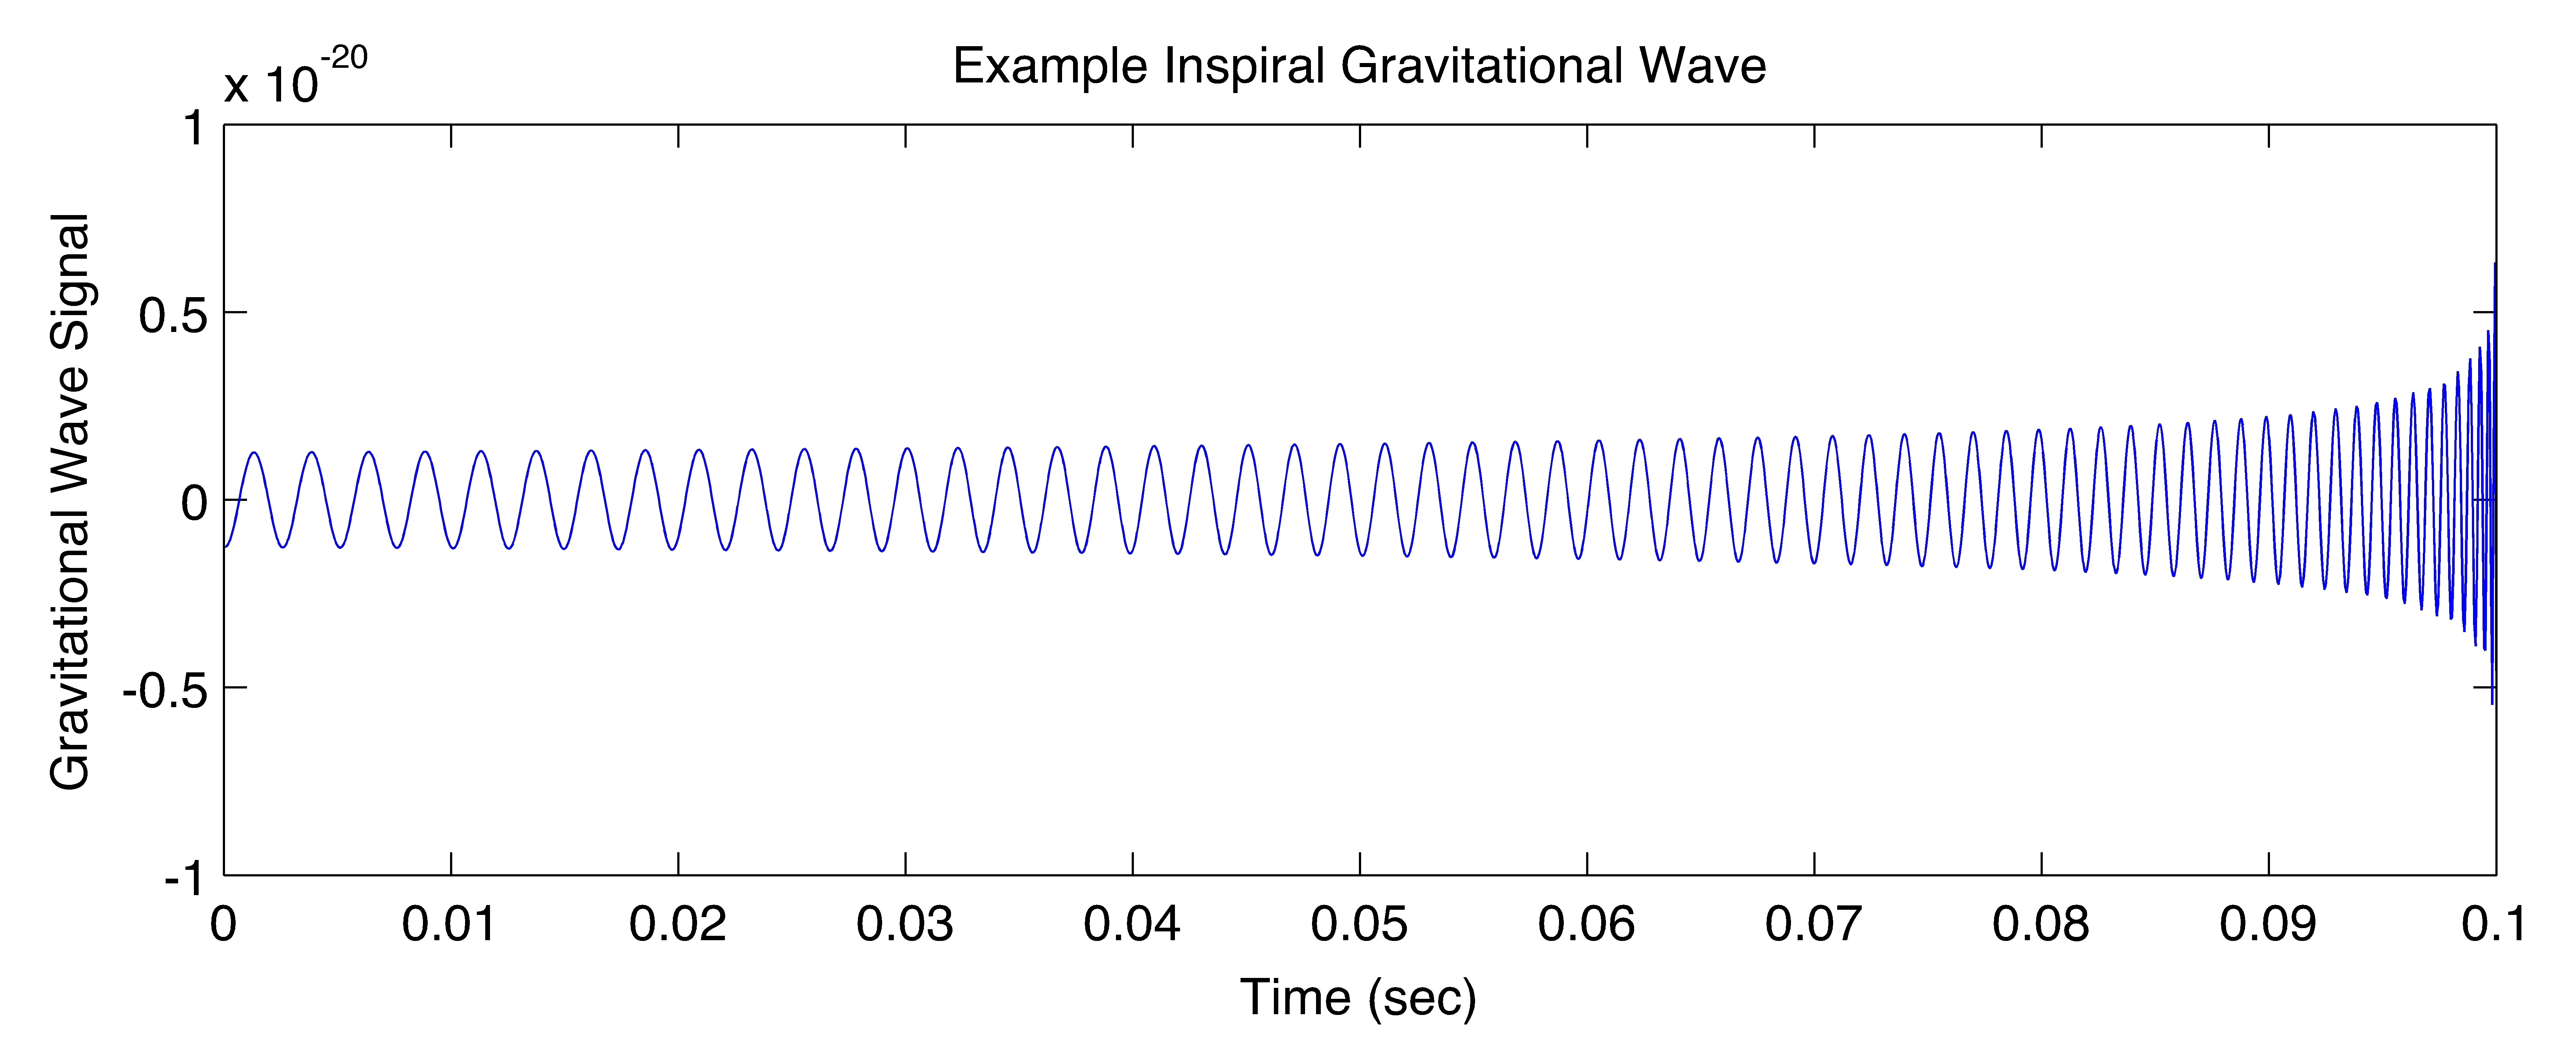
\includegraphics[scale=0.05]{Images/chirpT.png}
\caption{Time evolution of the strain $h(\tau)$ at the detector due to a \ac{GW} -- the ``chirp'' wave in time domain. This particular ``chirp'' is produced to first order by an ideally located and oriented CBC with equal masses and no spins.}
\label{chirpwaveT}
\end{figure}

In the analysis it is useful to write the waveform at the detector as:
\be h(\tau) = \frac{1 ~\mathrm{Mpc}}{D_{\mathrm{eff}}}\left(h_+\sin \left(\Phi(\tau)+ 2\varphi\right) + h_{\cross}\cos \left(\Phi(\tau)+ 2\varphi\right)\right)
\ee
%
where 

\be
D_{\mathrm{eff}} = \frac{D}{\sqrt{F^2_+(1+\cos^2 \iota)/4 + F^2_{\cross} \cos^2 \iota}}
\ee
%
is the effective distance to a binary given the antenna response factors $(F_+,~F_{\cross})$ and $h_+, ~h_{\cross}$ are the two polarizations for a binary ideally oriented and located.

One must remember that this waveform has only been generated to first order and without taking into account the spin of the component objects. For a real signal, higher order terms will be important close to merger. Additionally, the assumption of point masses will break down at merger, as effects due to the size of the objects, such as the tidal interaction between two neutron stars, can become noticeable.

\section{Gravitational Waves Detectors -- Practical Issues}
Suppose we consider a real gravitational wave interferometer with each of the ``L'' arms of 4 km long. The variation in ``L'' arm length to which a \ac{GW} interferometer should be sensitive in order to detect a \ac{GW} of strain amplitude $h \approx 10^{-21}$, given an arm length of 4 km follows from equation (\ref{varh_L}):

\begin{equation}
\Delta L \approx hL = 4 \times 10^{-18}~\mathrm{m}
\end{equation}

At such scales, one would expect that even the smallest amount of noise would drastically affect the sensitivity of a \ac{GW} interferometer. The time it takes light to travel along the arms is of order $10^{-5}$~s, much smaller than the duration of a gravitational wave. In order to enlarge this time, different optical components are used to keep the light longer in the arms. These optical parts will introduce their own sources of noise. Internal and external detector environment factors can contribute to both stationary and non--stationary noise effects and are briefly mentioned here.

\subsection{Stationary noise sources}

The main sources of stationary noise for a typical interferometric detector are given in various references and summarized here. For a more in--depth analysis of the topic we direct the reader to a few references, e.g., \cite{Saulson:1994, Sathyaprakash:2009xs, Blackburn:2008ah, Accadia:2010zzb, Accadia:2010zz}. Figure \ref{noisesF} shows the stationary noise contributions in the frequency regime for a GW detector.

\begin{figure}[ht!]
\centering
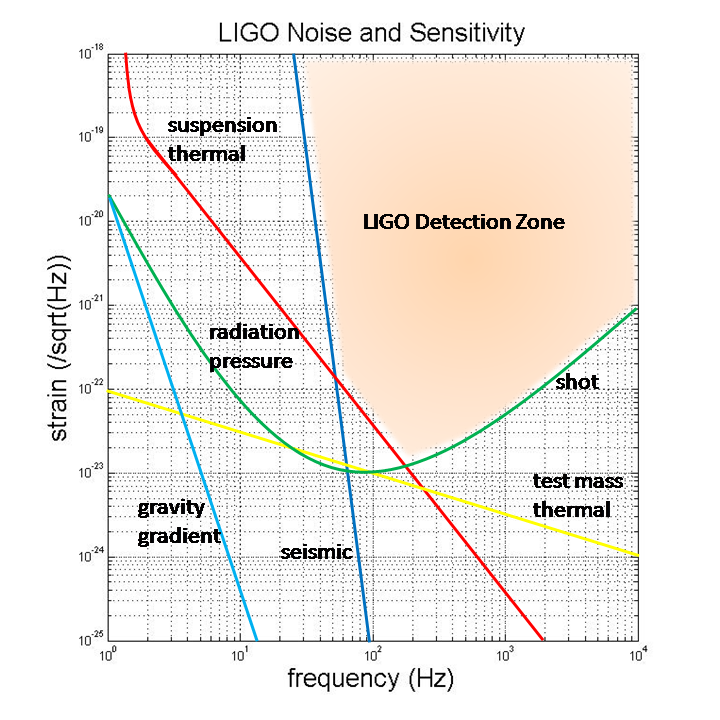
\includegraphics[scale=0.50]{Images/noisesF.png}
\caption{Different noise contributions in the frequency regime. Image from \cite{ian}.}
\label{noisesF}
\end{figure}

\begin{itemize}
 \item
   {\bf Thermal noise:} Thermal vibrations of the internal parts of the interferometer can mask gravitational waves. Interferometers minimize the effect of noise by measuring only at frequencies \emph{far} from the resonant frequency where the effects of thermal noise are maximum (suspensions have resonant frequencies of a few Hz, whereas mirrors' are at a few kHz, see Figure \ref{noisesF}). This noise source is also minimized by making sure all materials have high quality factors, which is technologically demanding, so their resonances are sharp and energy leakage to measurement frequencies is small. In terms of temperature, interferometers usually operate at room temperature. Alternatively the detector could be cryogenically cooled as proposed in the Japanese LCGT project \cite{lcgtwebsite}. For a reference on thermal noise please consult \cite{Gillespie:1993vg}.
 \item
   {\bf Shot noise:} The photons that are used for interferometry arrive with random phases at the photodetector. Therefore they introduce random fluctuations in the interference pattern that may mimic a gravitational wave signal (the photons are Poisson--distributed). The more photons one uses, henceby increasing the laser power, the smoother will be the interference signal.
  \item
  {\bf Mechanical vibration:} This source of noise is produced by internal vibrations of the mechanical components of the detector (primarily suspensions). Mechanical vibrations must be screened out; there are many different ways to do this, but all of them are very sensitive to frequency, working well down to a lowest effective frequency. The most ambitious isolation system is currently being developed for the Virgo detector.
 \item 
{\bf Radiation pressure:} Photons hitting the end mirrors exert a pressure on them proportional to the number and momentum of photons, moving it slightly and changing its optical contribution in the system. This noise source can be reduced by decreasing the power of the laser, thus reducing the number of photons and the total pressure. However, this will increase the shot noise. A balance must therefore be reached between the radiation pressure and the shot noise.
 \item
{\bf Seismic noise:} A very important source of noise in the low--frequency regime. Ground vibrations induced by seismic activity, man--made objects or even ocean waves may produce signals in the detector that look like very strong \ac{GW}. These vibrations act on the mirrors hence it is very important to isolate the mirrors as much as possible from the ground. The seismic noise will play an important role in the next generation \ac{GW} detectors that will operate at frequencies $\sim~4$ times lower than the present detectors. 
\end{itemize}

\subsection{Non--stationary noise sources}
The above list of noise sources enumerates only the stationary and \emph{predictable} sources of noise. More importantly, the non--stationary \emph{unpredictable} noise sources may induce large fluctuations in the detector output that may mimic strong \ac{GW} signals. These include any local small--time--scale disturbance produced by a noise transient, e.g., a truck passing near the detector will cause ground vibrations that will couple to mirror motion. There are a series of auxiliary channels that permanently monitor these noise sources and everytime there is excessive noise activity they will prompt the data to be discarded. Surviving non-stationary transients or ``glitches'' are often mistakenly picked up by the data analysis process as interesting events, therefore ``glitch''--rejection mechanisms are important and will be discussed in Chapters \ref{Chapter Three} and \ref{Chapter Four}.

\section{A network of gravitational waves interferometers} 
A global network of gravitational wave interferometers has now been constructed and has been taking data for the past ten years. The instruments constituting this network include the Laser Interferometry Gravitational Observatory (LIGO or, recently labelled as Initial LIGO), which operates two observatories at Hanford and Livingston in the USA \cite{Abbott:2007kv}; the French--Italian Virgo (Initial Virgo) detector based in Cascina, Italy \cite{virgo, Acernese:2006bj}; the British--German GEO600 detector, near Hannover in Germany \cite{Willke:2007zz} and the TAMA300 detector in Japan \cite{TAMA_status}. Initial LIGO and Virgo ceased their operations in 2010 and are both currently undergoing major upgrading work to become Advanced LIGO \cite{avlligowebsite, Harry:2010zz} and Advanced Virgo \cite{advvirgowebsite}, the second generation interferometric detectors with a much higher sensitivity than the initials.  The next subsections will briefly describe each of these detectors, for an in--depth analysis of their specifications and operational standards, we invite the reader to consult the listed references.  

\subsection{LIGO and Virgo detectors}

\ac{LIGO} (United States), is the largest interferometer in use as of today. LIGO operates two gravitational wave observatories (at two different sites) in unison: the LIGO Livingston Observatory in Livingston, Louisiana (L1 or LLO) and the LIGO Hanford Observatory, located near Richland, Washington (LHO, initially with two co--located and co--aligned detectors: H1 (4 km) and H2 (2 km)). These sites are separated by 3,002 km \cite{Abadie:2010px}. Each observatory supports an ``L''--shaped ultra high vacuum tube system, measuring 4 kilometers on each side. The primary interferometer at each site consists of mirrors suspended at each of the corners of the ``L''; it is known as a special Michelson interferometer in that it recycles the power. A pre--stabilized laser emits a beam of up to 35 W that passes through a beam splitter at the vertex of the ``L'' arms. There, the beam splits into two paths, one for each arm; each arm contains special cavities that store the beams and increase the effective path length by multiple reflections.

The Initial Virgo (Italy and France) is a 3 km detector located in Cascina, near Pisa, Italy. Virgo specializes in sophisticated suspensions, and the control of vibrational noise. Its goal is to observe at the lowest possible frequencies from the ground, at least partly to be able to examine as many pulsars and other neutron stars as possible.

The initial LIGO and Virgo took data in six consecutive science runs. Since the author has worked from the fifth run onwards as part of the LIGO Scientific Collaboration and Virgo Collaboration, we will try summarize the fifth and six runs only. The fifth science run was completed between November 4, 2005 and October 1, 2007 (known as S5 in LIGO/GEO and VSR1 in Virgo nomenclatures).  The detectors achieved a strain sensitivity of better than $10^{-22}/\sqrt{\mathrm{Hz}}$ at their most sensitive frequencies (around 100 Hz). This can be translated into sensitivities to various sources, for example the LIGO detectors in S5 were sensitive to optimally oriented and located binary neutron star coalescence signals to a distance of $\sim 35$ Mpc, and hundreds of Mpc for more massive compact binary mergers. For a better understanding of a detector sensitivity measure to GW inspiral signals from CBC objects, we invite the reader to consult Chapter \ref{Chapter Three}. For short--duration, narrow--band transients (bursts), such as the GW signal one may expect from core--collapse supernovae, this sensitivity corresponds to a gravitational wave energy as low as $10^{-8} M_{\odot}c^2 \sim 2 \times 10^{46}$~erg for galactic events and $0.1 M_{\odot}c^2 \sim 2 \times 10^{53}$~erg for events in the Virgo cluster at 16 Mpc.
%
\begin{figure}[ht!]
\centering
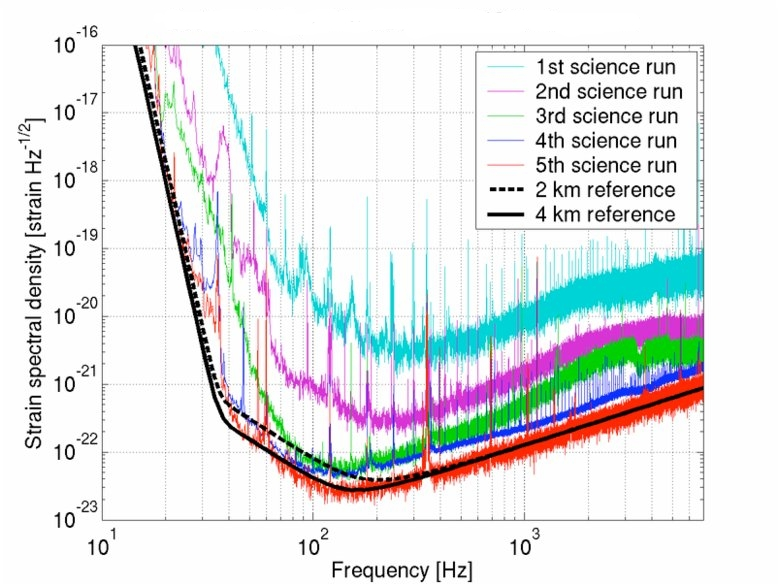
\includegraphics[scale=0.40]{Images/ligonoise.png}
\caption{LIGO noise curve for five consecutive science runs (S1 to S5): the detector sensitivity quantified by the strain spectral density is shown as function of signal frequency. The most sensitive region is around $f\sim100$ Hz. Image initially published in \cite{Abadie:2010yba}.}
\label{ligonoise}
\end{figure}

Following the S5/VSR1 run, the LIGO and Virgo detectors have been technically upgraded to enhanced configurations, and the latest completed science run was S6/VSR2 and 3 that began in the summer of 2009, and ended in fall 2010, aiming at collecting data at better sensitivities than the previous science runs (see Chapter \ref{Chapter Four}, Table \ref{tab:sciencetimes} for a complete list of dates for both S5/VSR1 and S6/VSR2 and 3).

The performance of a gravitational wave detector is characterized by the \emph{power spectral density} (or PSD) of its noise background. Although this quantity will be discussed in detail in Chapter \ref{Chapter Three}, we would like to introduce it here in light of characterizing detector sensitivity. A sensitivity curve for a detector, or a PSD curve, represents a detector strain vs. frequency plot for a frequency range for a series of noise sources. Such a curve is shown in Figure \ref{noisesF}. A collection of PSD curves for a number of GW interferometers is presented in Figure \ref{noisesmultiples}.

\begin{figure}[ht!]
\centering
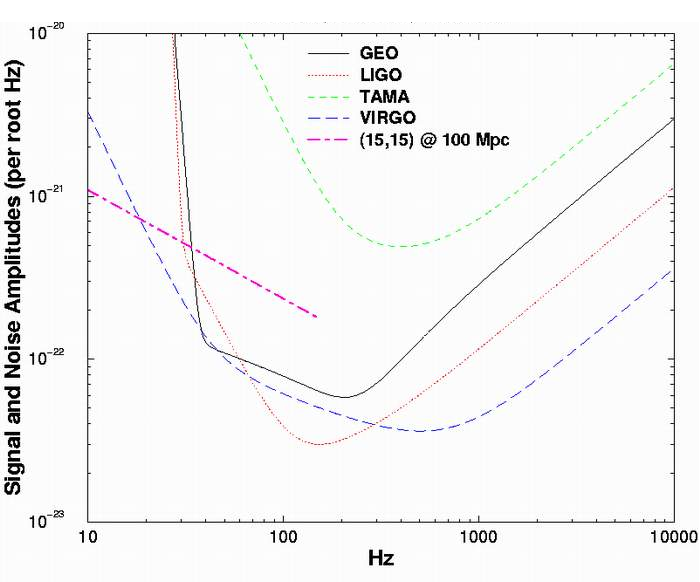
\includegraphics[scale=0.50]{Images/PSD_detectors.png}
\caption{Detector PSD curves, together with the inspiral signal evolution of a 15--15 $M_{\odot}$ compact binary at 100 Mpc. Image initially published in \cite{Abadie:2010px}}
\label{noisesmultiples}
\end{figure}

\subsection{The Advanced Detectors}

Following the initial LIGO and Virgo data taking period (S1 to S6 for LIGO and VSR1 to VSR2,3 for Virgo), both LIGO and Virgo detectors are being upgraded to advanced configurations to achieve approximately ten times the strain sensitivity (in distance) of the initial detectors. For sources distributed uniformly in volume, this corresponds to a sensitivity to a thousand times as many sources. In terms of energy, the sensitivity will be $\sim 10^{-10} M_{\odot}c^2 \sim 2 \times 10^{44}$~erg for galactic events. The low--frequency cut--off due to seismic noise will be lowered from 40 Hz to 10 Hz. The work towards completing the advanced detectors has started in 2011 and are expected to begin acquiring scientific data by no later than 2015 \cite{avlligowebsite,Harry:2010zz}.

Advanced LIGO will operate at such predicted sensitivity due to a series of radical changes from the initial detectors: the initial LIGO 10 W laser will be upgraded to a more powerful 180 W laser -- with this the input optics is changed as well, to match the new laser, improving the shot noise limited sensitivity by a factor of $\approx$ 6 with respect to Initial LIGO; the power--recycling will be more efficient as well, with changes applied to the power--recycling mirrors, resulting in a much reduced effect of thermal noise; a new suspension configuration will allow improved operation at low frequencies, where the dominant source of noise is seismic oscillations -- this way the low frequency cut--off is lowered to 10 Hz \cite{Waldman:2011vg}. 



\subsection{Sky localization with a network of \ac{GW} detectors}
\label{gw_skyloc}

Here we would like to briefly address the problem of localizing a \ac{GW} source, in case of a detection, using information from \ac{GW} detectors only. As we have seen above from equation (\ref{eq:h_amp_phase_freq}) a single detector cannot localize a \ac{GW} source. In turn, if we have two detectors, source localization could be achieved to a certain error region of the sky. \ac{GW} detectors, when working together in a \emph{network} of detectors, localize sources by \emph{triangulation} \cite{Fairhurst:2009tc}. This is possible due to differences in times of arrival of the same \ac{GW} signal at different detector sites. Indeed, if we consider two detectors (1,2) separated by a linear geographical distance ${\bf S}$ and a \ac{GW} source at a distance ${\bf R}$ on the celestial sphere, the expected time difference of signal arrival at the two detectors will be:
%
\be \Delta t_0 = t_{01} - t_{02} = \mathbf{S} \cdot \mathbf{R} \ee
%
This time delay is called the \emph{light travel time} -- the expected time difference it takes a gravitational wave to be recorded at both detector sites. We have to note that these are \emph{expected} times in the case of an ideal detector. Since the detectors are affected by noise (see Chapter \ref{Chapter Three}) the times $t_{01}, ~t_{02}$ are in reality distributed in a discrete region. \ac{GW} detectors have a relatively poor capability of determining the sky location for a source, as compared with, for example, other \ac{EM} telescopes: the angular resolution of the source can extend to thousands of square degrees; with three or more detectors the resolution will decrease to a few square degrees \cite{Fairhurst:2009tc, Fairhurst:2010is}.

